\chapter{Studying cognition with task-based fMRI: reality filtering in young populations}\label{chapter:ch4}


\vspace{2cm}

While resting-state studies provide insightful information on spontaneous brain function, task-based functional magnetic resonance imaging (fMRI) paradigms are essential to probe into brain activation driven by specific demands. As described in more detail in this chapter, the prefrontal cortex --- specifically the orbitofrontal cortex (OFC) --- has been shown to be essential for the ability to process reality filtering tasks in adults \citep{Schnider2018}. This region is, however, known to be underdeveloped in preterm-born individuals \citep{Thompson2007}. The goal of this chapter is thus twofold: to investigate whether, as in adults, the OFC mediates reality filtering in young adolescents; and whether preterm-born young adolescents use the same brain resources as fullterm-born controls to perform a reality filtering task.  


The first article included in this section has been published in the peer-reviewed Brain and Behaviour journal. Its goal was to test the hypothesis that the OFC mediates reality filtering processing in young adolescents. Maria Chiara Liverani and Lorena Freitas are considered joint first-authors for the paper, having performed the behavioural and neuroimaging analyses, respectively. In addition, Liverani and Freitas both participated in data collection for this study. The remaining authors participated in different stages of ideation for the overarching project (\textit{Building the Path to Resilience in Preterm Infants}) and/or provided funding. 

The second article is a preprint of the followup study looking into reality filtering in preterm-born children as compared to the control group from the first study. 

\clearpage

\section{Journal Article:  Get real: orbitofrontal cortex mediates the ability to sense reality in early adolescents} \label{section:ch4_orfi_ctrl}

\begin{center}
\textit{(Postprint version of the article published in: Brain and Behaviour, 2020,  DOI:~https://doi.org/10.1002/brb3.1552)}

Maria Chiara Liverani*\textsuperscript{1}, Lorena G. A. Freitas*\textsuperscript{1,2}, Vanessa Siffredi\textsuperscript{1,2}, Greta Mikneviciute\textsuperscript{1}, Roberto Martuzzi\textsuperscript{3}, Djalel-Eddine Meskaldij\textsuperscript{1,4}, Cristina Borradori Tolsa\textsuperscript{1}, Russia Ha-Vinh Leuchter\textsuperscript{1}, Armin Schnider\textsuperscript{5}, Dimitri Van De Ville\textsuperscript{2}, Petra S. Hüppi\textsuperscript{1}

\textit{* M.C.L. and L.G.A.F. have contributed equally and are considered joint-first authors.}

\end{center}

\textsuperscript{1} Department of Paediatrics, Gynecology and Obstetrics, Division of Development and Growth, Geneva University Hospitals, 6 rue Willy – Donzé, 1205 Geneva, Switzerland \\
\textsuperscript{2} Institute of Bioengineering, École Polytechnique Fédérale de Lausanne, Rue Cantonale, 1015 Lausanne, Switzerland  \\
\textsuperscript{3} Foundation Campus Biotech Geneva, Chemin des Mines 9, 1202 Geneva, Switzerland  \\
\textsuperscript{4} Institute of Mathematics, École Polytechnique Fédérale de Lausanne, Rue Cantonale, 1015 Lausanne, Switzerland  \\
\textsuperscript{5} Department of Clinical Neurosciences, Division of Neurorehabilitation, Geneva University Hospitals, 26 Avenue de Beau-Séjour, 1211 Geneva, Switzerland  \\

\subsection*{Abstract}

Introduction: Orbitofrontal reality filtering (ORFi) is a memory mechanism that distinguishes if a thought is relevant to present reality or not. In adults, it is mediated by the orbitofrontal cortex (OFC). This region is still not fully developed in pre-teenagers, but ORFi is already active from age 7. Here we probe the neural correlates of ORFi in early adolescents, hypothesizing that OFC mediates the sense of reality in this population.

Methods: Functional magnetic resonance images (fMRI) were acquired in 22 early adolescents during a task composed of two runs: Run 1 measuring recognition capacity; Run 2 measuring ORFi; each containing two types of images (conditions): distractors (D: images seen for the first time in the current run) and targets (T: images seen for the second time in the current run). Group region of interest (ROI) analysis was performed in a flexible factorial design with two factors (run and condition) using SPM12. 

Results: We found significant main effects for the experimental run and condition. The bilateral OFC activation was higher during ORFi than during the first run. Additionally, the OFC was more active while processing distractors than targets. 

Conclusion: These results confirm, for the first time, the role of OFC in reality filtering in early adolescents.

Keywords: \textit{Orbitofrontal reality filtering, fMRI, orbitofrontal cortex, early adolescents, memory.}

\subsection{Introduction}

Orbitofrontal reality filtering (ORFi) is a memory control mechanism that allows to filter upcoming memories and thoughts according to their relation with ongoing reality \citep{Schnider2013,Schnider2018}. The first description of ORFi was based on the observation of patients with orbitofrontal lesions, suffering from behaviourally spontaneous confabulations and disorientation. These patients typically act to currently inappropriate memories to guide their present actions or to shape their future plans, failing to verify the connection of these memories with the “now”. In addition, they are disoriented in time and space \citep{Schnider2018}.  For example, a retired psychiatrist hospitalised after rupture of an aneurysm of the anterior communicating artery, repeatedly tried to leave the hospital in the conviction that she had to meet her own patients \citep{Schnider2005}. 
Schnider and colleagues \citep{Schnider1996} developed an experimental paradigm to test ORFi and to reliably discriminate reality-confusing patients from healthy participants. It consists of two runs of a continuous recognition task in which the same images are shown twice. Participants are asked to indicate picture recurrences only within the ongoing run. The first run assesses the ability to encode and recognize items, and familiarity alone is sufficient to correctly perform the task. In the second run all images are familiar, and thus familiarity alone is not enough to perform the task. In this second run ORFi is needed, representing the ability to sense whether the memory of an item relates to the present (the currently ongoing run), or not \citep{Schnider1999}. 

Behaviourally, confabulating patients markedly and specifically increased their false positives in the second run \citep{Nahum2012, Schnider1999}. Lesion analysis on these patients revealed that the ORFi mechanism depends on the orbitofrontal cortex (OFC) or structures directly connected with it \citep{Schnider1996, Schnider2018}. Functional neuroimaging studies using Positron Emission Tomography further corroborated the dependence of ORFi on the intact OFC  \citep{Schnider2000,Treyer2003,Treyer2006}. Electrophysiological studies revealed that ORFi is expressed by a frontal positivity at about 200-300 ms, before the content of a thought is recognised \citep{Schnider2002}.

Children are more vulnerable to memory distortions and more prone to errors than adults \citep{Ceci1993}. Using a child-adapted version of the continuous recognition task, we recently found that ORFi is present in 7-year-old children, improves from 7 to 11 years in parallel with memory capacity, but does not attain adult efficacy at that age \citep{Liverani2017}.

The neural correlates of this mechanism in children and adolescents has never been investigated. While the implication of the OFC in ORFi has clearly been shown in adults \citep{Treyer2003,Treyer2006}, no such evidence exists in a younger population. 

The aim of this study was to examine, with advanced functional neuroimaging techniques, to which extent the ability of early adolescents to sense whether a memory or a thought refers to the present reality or not depends on the OFC, similar to what has been found in adults. 


%% METHODS
%% ----------------------------------------------------------------------
\subsection{Methods}

\subsubsection{Participants} \label{subsection:OFC_participants}
Twenty-three healthy early adolescents from 10 to 13 years of age (10 females, mean age 12 $\pm$ 1.01 years) were recruited through advertisements. One participant was excluded due to strong signal distortions on fMRI images caused by the subject’s dental braces.  Twenty-two participants were finally included in the analysis.

Cognitive assessment at the time of the scan was performed using the French version of the Wechsler Intelligence Scale for Children – Fifth Edition (WISC - V; \citeauthor{Wechsler2014}, \citeyear{Wechsler2014}). For one participant IQ score was evaluated using the Kaufman Assessment Battery for Children, second edition (KABC-II; \citeauthor{Kaufman2004}, \citeyear{Kaufman2004}). All participants scored within the normal range of intellectual functioning (mean = 117.04 $\pm$ 11.35). Parents were asked to fill a questionnaire assessing the presence of serious physical illness or neurological problems. None of the participant had major disabilities, psychiatric or neurological diseases.

The Ethics Committee of the Canton of Geneva approved the study, which was carried out in accordance with the Declaration of Helsinki. Caregivers and participants provided informed written consent. Participants received a gift voucher of 100 Swiss francs for their participation in the study. 

\subsubsection{fMRI Paradigm} \label{subsection:OFC_paradigm}
Participants performed a child-adapted version of the continuous recognition task assessing recognition memory and orbitofrontal reality filtering (Figure \ref{fig:taskDesign}; \citeauthor{Liverani2017}, \citeyear{Liverani2017}; \citeauthor{Schnider1996}, \citeyear{Schnider1996}; \citeauthor{Schnider2003}, \citeyear{Schnider2003}, \citeyear{Schnider2013}), associated with an event-related fMRI paradigm.


\begin{figure}[h]
\centering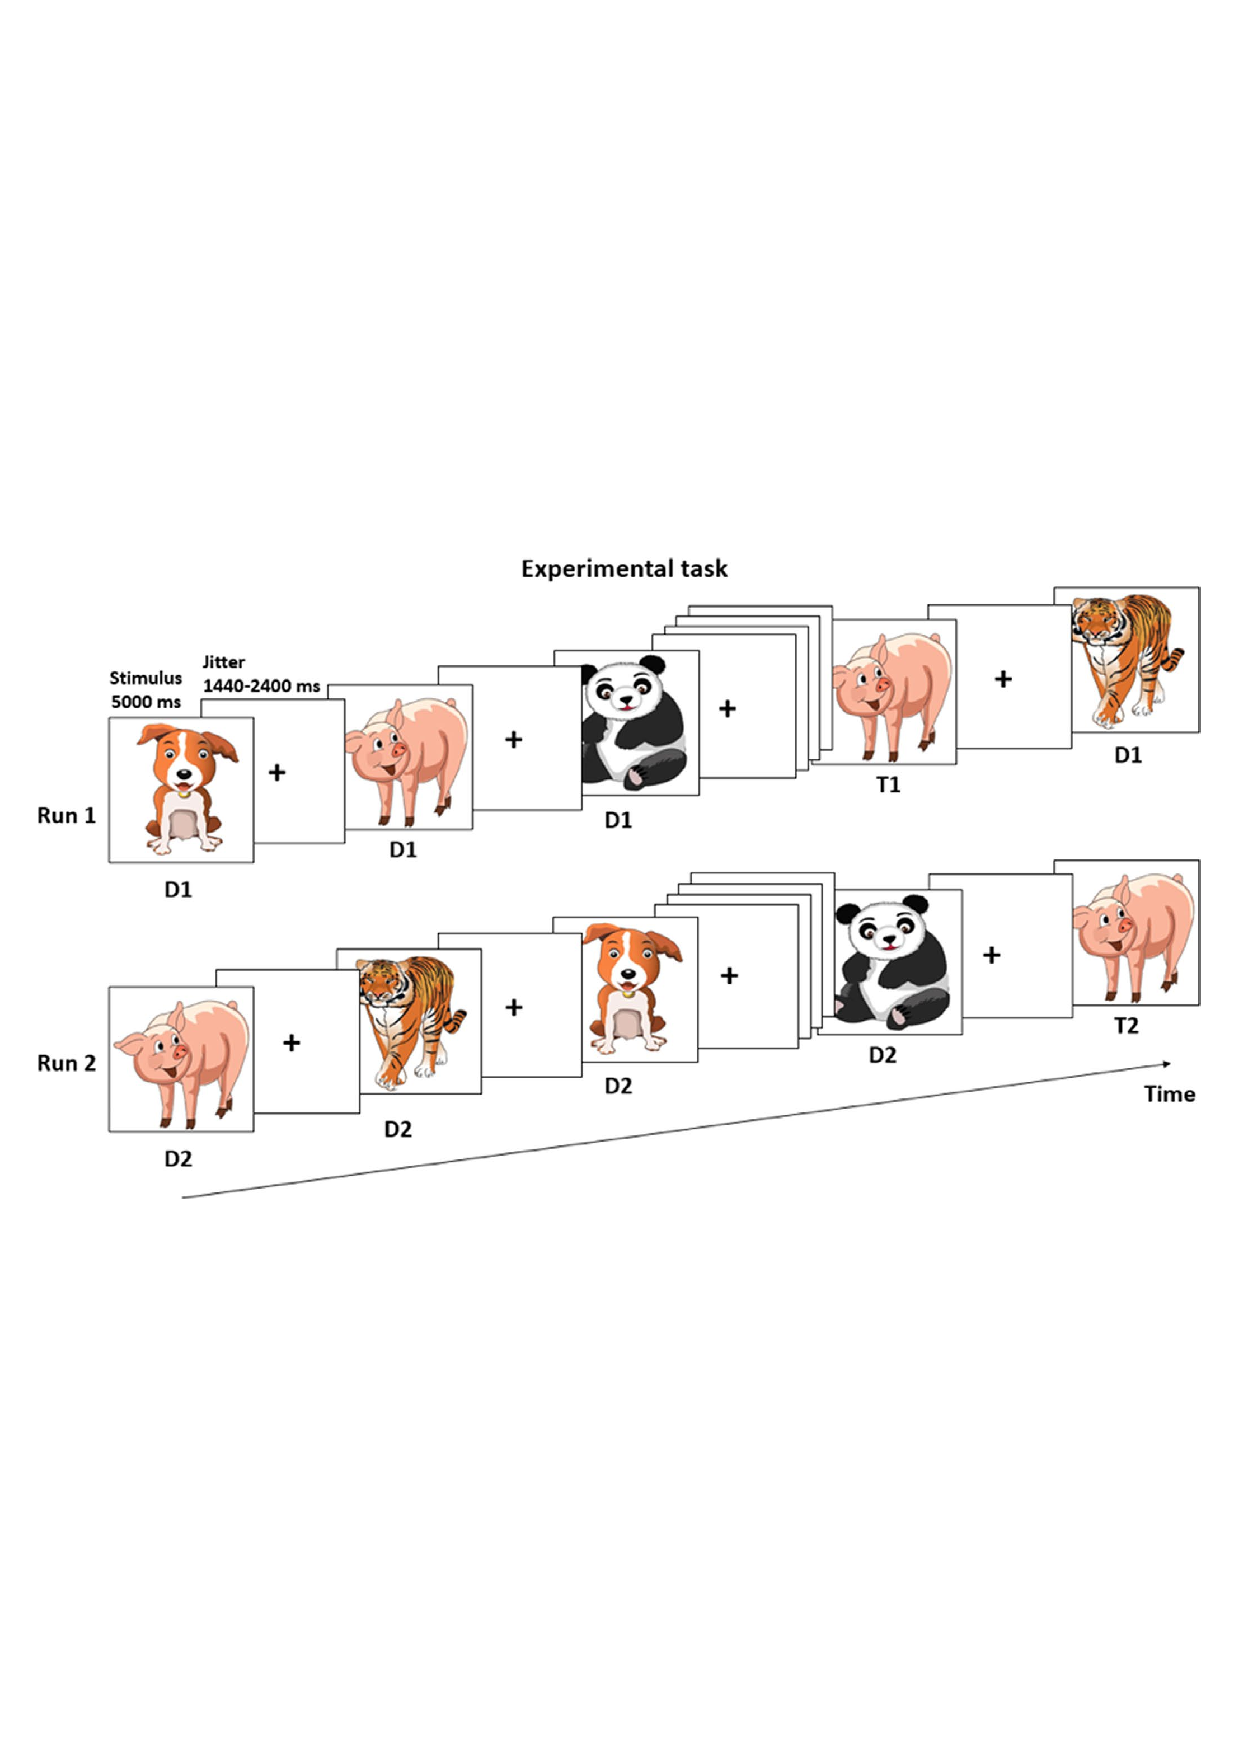
\includegraphics[width=1\linewidth]{images/Ch4/Figure1_fMRIparadigm.pdf}
\caption{\textbf{Task design. }  The task was composed of 2 runs, separated by a break of 3 minutes. Distractors (D1, D2) are images presented for the first time within a run; targets (T1, T2), are images repeated within the same run.}
\end{figure} \label{fig:taskDesign}






The task was composed of two runs in which the same set of images was presented and repeated twice, with a break of around 3 minutes between the two runs. In the first part, assessing recognition memory (item recognition, IR) participants were asked to indicate picture recurrence ("Have you already seen this picture in this task?”) by pressing the left button of an MRI-compatible mouse if the image was seen for the first time (distractors run 1, D1), and the right button if it was seen for the second time (targets run 1, T1). This run can be solved on the basis of familiarity alone. In the second run, the same set of pictures was presented in a different order and repeated twice. Participants were instructed to indicate if each item was presented for the first or the second time in this ongoing run ("Is this the first or the second time that you see that image in this ongoing run?"), pressing the left button of the mouse for images seen for the first time (distractors run 2, D2), and the right button for images presented for the second time (targets run 2, T2). In this run all images have already been seen. Therefore, familiarity alone is not enough to correctly perform the task, and the ORFi mechanism is needed to process distractors (D2).

Pictures were a set of 30 cartoon drawings of animals and were presented for 5 seconds on the screen. In each run, 30 images were presented for the first time (distractors, D) and then repeated once (targets, T) after 6 to 9 intervening pictures, has already done in a previous study with children \citep{Liverani2017}. After each image, a fixation cross was presented during between 1440 and 2400 milliseconds. Each run lasted approximately 7.5 min. Stimuli were displayed on a white screen at the head of the scanner via a 45° angled mirror fixed to the MRI head coil. Responses were given by pressing two buttons with the right index and middle finger, on an MRI-compatible mouse. Task programming, stimuli display and responses logging were done using E-Prime 2 (Psychology Software Tools, Pittsburg, USA). All participants successfully completed a short training with a different set of images in the mock MRI scanner before the MRI.

\subsubsection{Behavioural data analysis} 
Reaction times and accuracy were recorded for each condition (D1, T1, D2, T2). A 2 X 2 repeated measures analysis of variance (ANOVA) was performed on accuracy and reaction time with the within-subject factors Run (1, 2) and Stimulus (distractor D, target T). 

\subsubsection{Image acquisition} \label{section:OFC_imgAcquisition}
MRI data were acquired on a Siemens 3T Magnetom Prisma scanner at Campus Biotech, Geneva, Switzerland. Structural T1-weighted MP-RAGE (Magnetization Prepared Rapid Gradient Echo) sequences were acquired using the following parameters: voxel size = 0.9 x 0.9 x 0.9 mm; repetition time (TR)~=~2300 ms; echo time (TE) = 2.32 ms; inversion time (TI) = 900 ms; flip angle (FA)~=~8°; field of view (Fov) = 240 mm. Functional images were T2*-weighted with a multislice gradient-echo-planar imaging (EPI) sequence of 64 slices; voxel size = 2 x 2 x 2 mm; TR = 720 ms; TE = 33 ms; Fov = 208 mm. Finally, a fieldmap was acquired each time a participant entered the scanner, with TR = 627 ms; TE1 = 5.19 ms; TE2 = 7.65 ms; and FA = 60°.


\subsubsection{MRI data preprocessing}  \label{section:OFC_preprocessing}
Our data were preprocessed using SPM12 (Wellcome Department of Imaging Neuroscience, UCL, UK) in Matlab R2016a (The MathWorks, Inc., Natick, Massachusetts, United States). One particular challenge in studying frontal brain areas using fMRI is the considerable vulnerability of these regions to signal distortions caused by field inhomogeneities around the air-filled sinuses \citep{Gorno-Tempini2002}. To correct for the resulting geometrical distortions, a field map was calculated from an additional stock double-echo field map sequence included in our MRI protocol \citep{Hutton2002}. The fMRI images from each participant were then spatially realigned and unwarped, respectively, to correct for motion artefacts and potential geometric distortions. Thanks to the distortion correction of vulnerable brain regions on the single-subject level, this additional unwarping step not only improves the co-registration between structural and functional images, but it also reduces the distortion variability across subjects during spatial normalization to a common space \citep{Hutton2002}.  This solution has been successfully used in several recent studies in adults including task \citep{Daw2011} and resting-state \citep{Togo2017} experimental paradigms, as well as in presurgical planning \citep{LimaCardoso2018} and in children \citep{Wozniak2011}.

In general, total head motion was very low on our participants as measured by Framewise Displacement (FD; \citeauthor{Power2014a}, \citeyear{Power2014a}): for the first fMRI run the mean FD per frame was 0.16 mm with a standard deviation (SD) of $\pm$ 0.04 mm; for the second run the mean FD was 0.15 mm $\pm$ 0.05 mm. Therefore, no participant was excluded due to high motion. Functional images were then coregistered to structural images in subject space and smoothed with a Gaussian filter of full width at half maximum (FWHM) = 6 mm. To be able to perform a group level comparison, data were warped into MNI (Montreal Neurologic Institute) space via a study-specific DARTEL (Diffeomorphic Anatomical Registration using Exponentiated Lie algebra) template. Normalisation methods such as these have been demonstrated to be robust to age differences in participants of 7 years and above \citep{ASHBURNER1998, Burgund2002}. Additionally, the inclusion of the DARTEL template as an intermediate step is among the top ranked currently available deformation algorithms \citep{Klein2009}. 

\subsubsection{Region of Interest (ROI analysis)} \label{section:OFC_ROIanal}
Statistical analyses were performed using SPM12 scripts implemented in Matlab R2016a in a two-step process, so that both intra and inter-subject variance were taken into account \citep{Friston1995a}. First-level (subject level) analyses were assessed on a voxel-wise basis using a General Linear Model (GLM). Within each condition, trials responded correctly and incorrectly were pooled together to generate the corresponding regressors. This was motivated by two main reasons: 1) this would ensure a similar number of trials per condition, and 2) our participants had consistently high rates of correct responses, which characterises a ceiling effect as discussed later. The condition regressors were produced by convolving SPM12’s canonical hemodynamic response function (HRF) with the onsets of each trial in an event-related design and included as regressors-of-interest in the individual design matrix. To further account for potential individual movement effects, we included in our model covariates-of-no-interest calculated in the following fashion: first, we computed the 24-parameter Volterra Expansion (VE) of the 6 motion parameters stored during the realignment step of the preprocessing pipeline. Secondly, we extracted the top 6 components (or those that explained 95\% of the variance in the VE) via singular value decomposition (SVD). Then, we included these components as nuisance regressors in the subject-level design matrix. This approach has been successfully used on our previous analyses of child data (see \citeauthor{Adam-Darque2018}, \citeyear{Adam-Darque2018} for an example). Finally, we employed the scan-nulling strategy \citep{Lemieux2007} to ignore information contained in fMRI images in which FD > 0.5mm, by adding extra regressors-of-no-interest for each of these time points.

The first-level results from all participants were then used in a second-level (group level) analysis in a factorial design with two factors (run and condition) with two levels each (2 runs and 2 types of stimuli, namely distractor and target). This design provides the flexibility to analyse main effects as well as a possible interaction effects between the factors. Given the a priori hypothesis of the involvement of the OFC in the reality filtering task based on neuropsychological data, lesion studies and PET imaging studies \citep{Schnider1996, Schnider1999, Treyer2003} , we performed an ROI analysis based on this brain region. Our ROI mask was defined as follows:  first, we downloaded a z-scored mask from NeuroSynth \citep{Wager2011a}, which was calculated as a meta-analysis of 665 independent studies for the term “orbitofrontal cortex”. This initial mask (nMask) was thresholded at z-value > 3, which is equivalent to a p-value < 0.001, and the largest continuous cluster was maintained. The nMask covered the entire bilateral OFC and can be seen highlighted in yellow in Figure \ref{fig:ROI}. Last, to ensure an equal contribution of all subjects to the analysis, we created a final mask (iMask) calculated as the intersection of all voxels within nMask that were present in the grey matter of every subject in our dataset. This can be seen as the blue highlight in Figure \ref{fig:ROI}. The contrast values for voxels within the ROI iMask from each subject were then averaged, and the resulting value entered in a 2-way analysis of variance (ANOVA). This strategy has two main advantages: it increases the signal to noise ratio, which improves the power of detecting true signals, and avoids the problem of multiple testing inherent in massive univariate approaches \citep{Benjamini2007, Meskaldji2015}. Although the ANOVA allows us to identify main, as well as interaction effects, it does not describe the effect’s direction – for example, it may tell us that the means between conditions are different, but not which one is greater. Thus, we performed additional t-tests within factors to clarify the direction of the effects found with the ANOVA and report the corresponding p-values, Bonferroni corrected for the number of effects that we find. Furthermore, in order to provide an estimate of each voxel’s contribution to the effects detected by these tests, we calculated the voxelwise t-values within the ROI.



\begin{figure}[h] 
\centering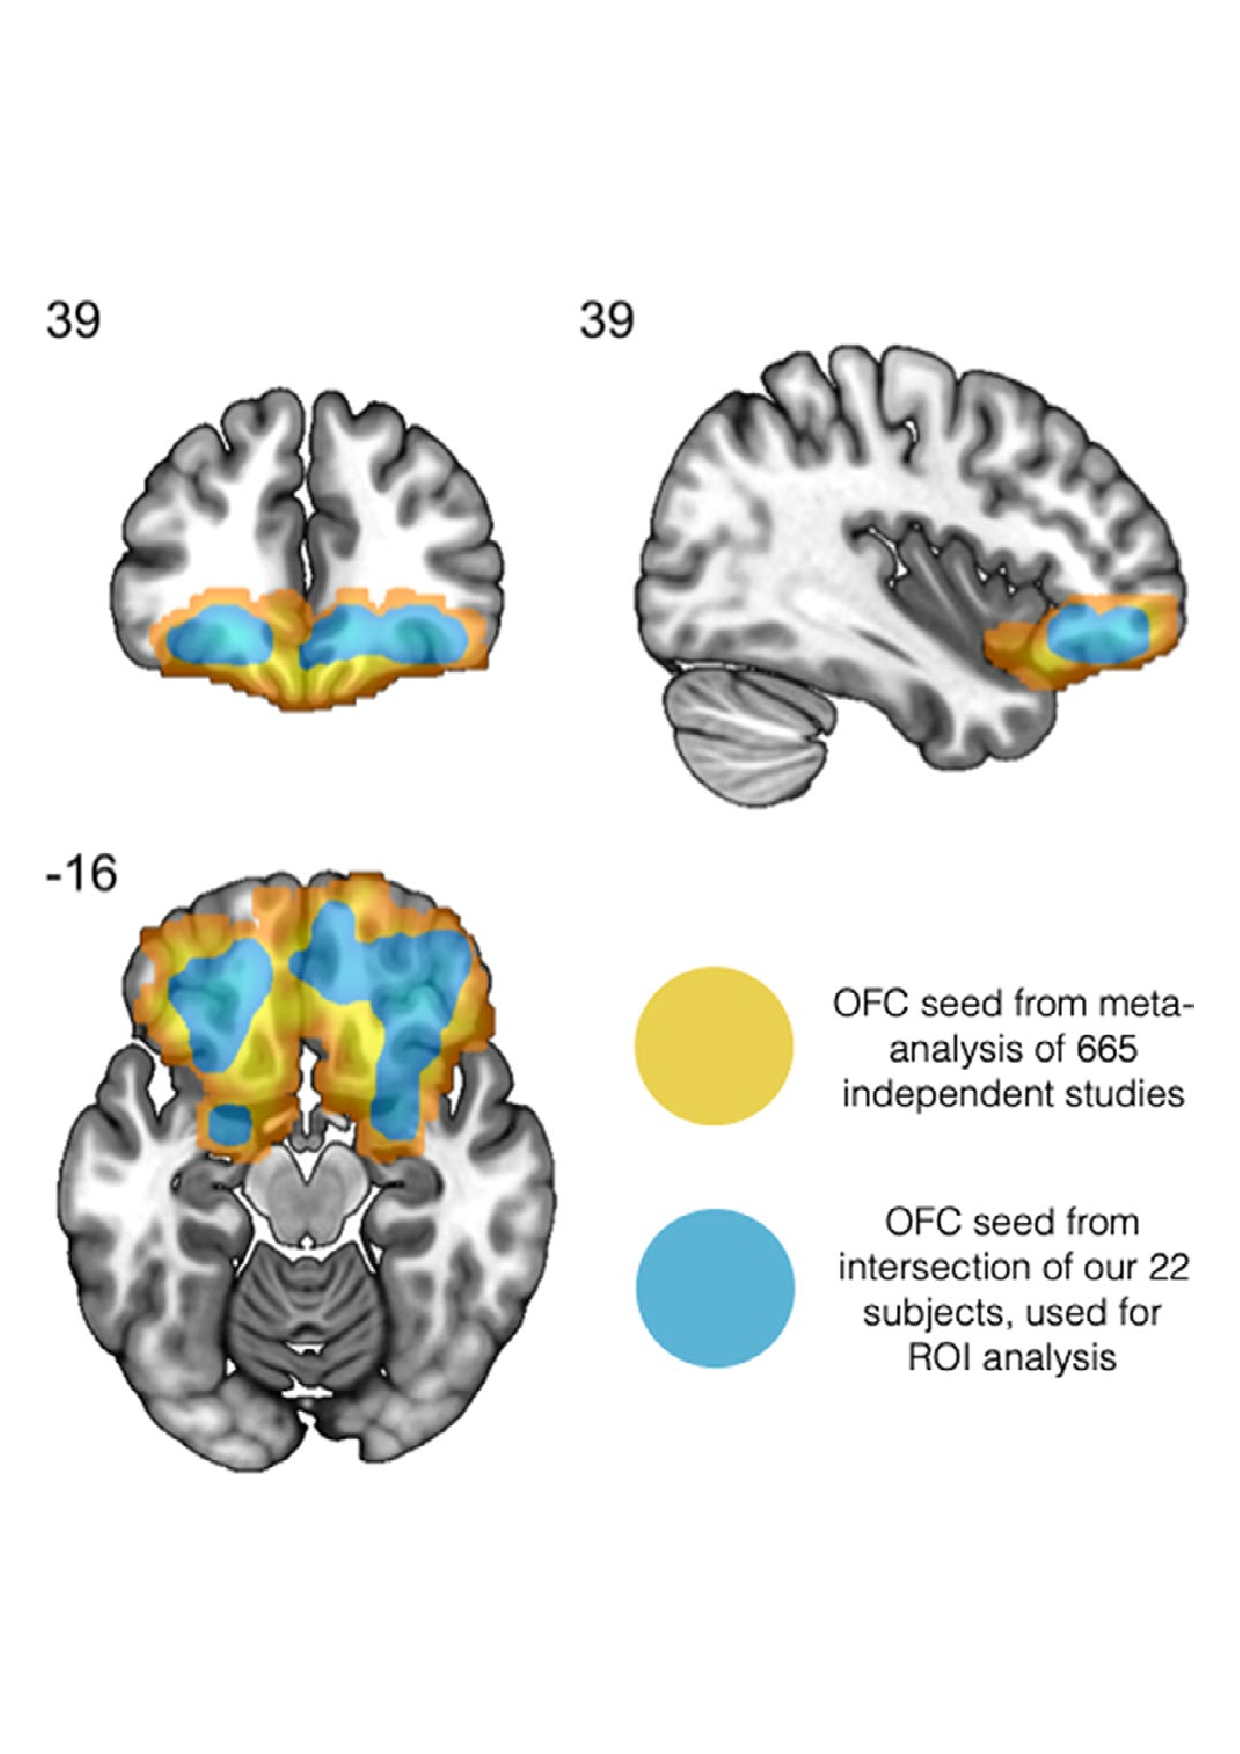
\includegraphics[width=0.7\linewidth]{images/Ch4/Figure2_ROI.pdf}
\caption{\textbf{The shaded areas show the orbitofrontal cortex ROI.  }   The region highlighted in yellow indicates the initial mask calculated from 665 independent studies using NeuroSynth. The area highlighted in blue corresponds to the intersection of grey matter voxels available for all participants within the initial mask. The latter was the final ROI used for this study. Brain images follow the neurological convention (left side shown on the left; right side shown on the right).} \label{fig:ROI}
\end{figure}


%% RESULTS
%% ----------------------------------------------------------------------
\subsection{Results}

\subsubsection{Behavioural results}

Behavioural descriptive results on accuracy and reaction times are summarised in Table \ref{tbl:stimulus}. Overall, a ceiling effect was found for the task accuracy, since participants had a very high rate of correct responses. The 2 X 2 repeated measures ANOVA on reaction times revealed a significant main effect of the factor Run (F\textsubscript{(1, 21)} = 12.14, p < 0.005, $\eta$\textsubscript{p}\textsuperscript{2} = 0.366), with faster responses for the first compared to the second run. No significant difference was found between Distractors and Targets reaction time (F(1, 21) = 0.001, p = 0.977, $\eta$\textsubscript{p}\textsuperscript{2} = 0.000). The interaction between the factor Run and the factor Condition was not significant.

\begin{table}
\begin{center}
\begin{tabular}{ ||l||c c|| } 

  \hline
\rowcolor{BabyBlue}
Stimulus type & Correct responses, \% (SD) & Reaction times, ms (SD) \\
  \hline
  \hline
Distractor, Run 1   & 96.06 (4.78) & 1454 (406) \\ 
  \hline
Target, Run 1      & 90.30 (16.93) & 1454 (369) \\ 
  \hline
Distractor, Run 2  & 93.63 (6.24) & 1579 (339) \\ 
  \hline
Target, Run 2      & 89.39 (13.97) & 1577 (413) \\ 

 \hline
\end{tabular}
\end{center}
\caption{Descriptive statistics of behavioural results on the reality filtering task. \textit{Distractor, Run 1} and \textit{Distractor, Run 2} are images seen for the first time in the first and in the second run, respectively. \textit{Target, Run 1} and \textit{Target, Run 2} are images seen for the second time in the first and in the second run, respectively.} \label{tbl:stimulus}
\end{table}




Accuracy analysis revealed no difference between the two runs (F \textsubscript{(1, 21)} = 1.36, p = 0.257, $\eta$\textsubscript{p}\textsuperscript{2}~=~0.061), as well as no difference between Distractors and Targets (F\textsubscript{(1, 21)}~=~3.14, p~=~0.91, $\eta$\textsubscript{p}\textsuperscript{2}~=~0.13). The interaction between the factor Run and the factor Condition was not significant. Violin plots in Figures \ref{fig:Fig3} and \ref{fig:Fig4} show the distribution of correct responses and reaction times for each condition, respectively. 




\begin{figure}[h] 
\centering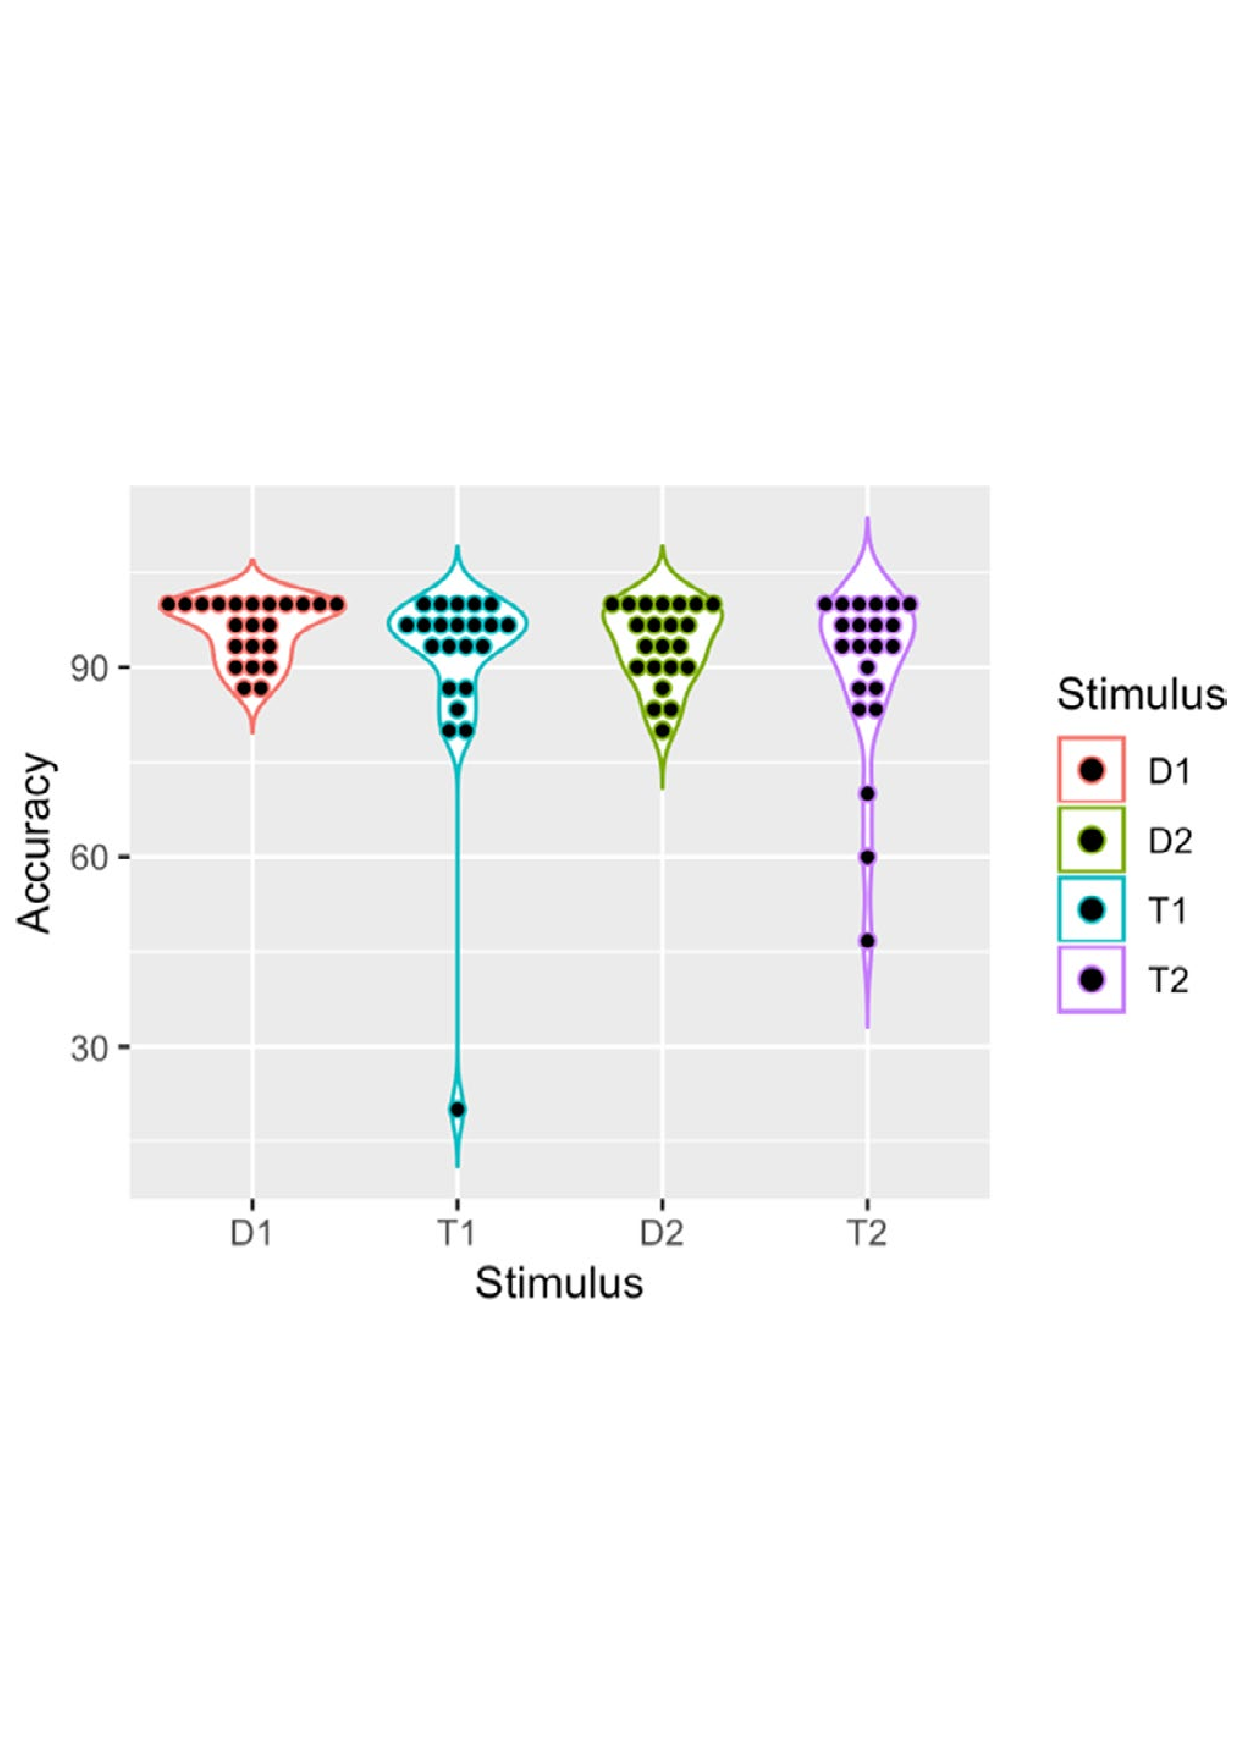
\includegraphics[width=0.7\linewidth]{images/Ch4/Figure3_Violin.pdf}
\caption{\textbf{Accuracy distributions by stimulus type.  }   The violin plots show the accuracy distribution per stimulus in the population. D1 = Distractor images in Run 1; T1 = Target images in Run 1.} \label{fig:Fig3}
\end{figure}



\begin{figure}[h]
\centering\includegraphics[width=0.7\linewidth]{images/Ch4/Figure4_Violin.pdf}
\caption{\textbf{Reaction Times by stimulus type.  }   The violin plots show the distribution of participant-averaged reaction times per stimulus in the population. D1 = Distractor images in Run 1; T1 = Target images in Run 1.}  \label{fig:Fig4}
\end{figure}






\subsubsection{ROI task-related activity}
To investigate whether there were main effects of run or condition, or an interaction between the two in the OFC, we first ran a 2-way ANOVA test (see Table \ref{tbl:anova}).  We found a significant main effect for the experimental “run” (F (1, 21) = 556.65, p = 0.027). Additionally, we found a significant main effect of the factor “condition” (F (1, 21) = 1014.64, p = 0.02). The interaction effect between run and condition was non-significant. 

\begin{table}
\vspace{20px}
\begin{center}
\begin{tabular}{ ||l||c c c|| } 

  \hline
\rowcolor{BabyBlue}
Factors & Mean Squared & F-statistic & p-value\\
  \hline
  \hline
Run   & 1.3219 & 556.65 & 0.027 \\ 
  \hline
Condition  & 2.4095   & 1014.64 & 0.02 \\ 
  \hline
Run * condition  & 0.0024 & 0 & 0.9455 \\ 

 \hline
\end{tabular}

\end{center}
\caption{2-way ANOVA with factors "run" and "condition" for brain activations in the orbitofrontal cortex. Run = Run 1 and Run 2; Condition = Distractors and Targets. } \label{tbl:anova}
\end{table}


We next sought to clarify the direction of the effects found from the ANOVA test. To this end, we first carried out a t-test comparing Run 2 and Run 1 (see Table \ref{tbl:posthoc}). As we hypothesised that the mean activation of the OFC during Run 2 would be higher than during Run 1, we first performed a one-tailed test. Indeed, we found that the overall bilateral OFC activation was higher during the Run 2, which specifically assess the reality filtering mechanism, than during Run 1 (T (21) = 2.12, p\textsubscript{(bonf)} = 0.04). Secondly, we performed a one-tailed t-test to compare the condition levels, with the hypothesis that the OFC would present a higher activity while processing distractors (D) than targets (T) all Run 1 and Run 2 together. This effect was also highly significant (T (21) = 3.70, p\textsubscript{(bonf)} = 0.0006). The comparison between D2 and T2 (distractors and targets from the second run, respectively) showed that their means were also significantly different in the same direction (T (21) = 2.41, p = 0.01). Figure \ref{fig:voxelwise} shows the voxelwise contribution to these results. 



\begin{table} 
\vspace{20px}
\begin{center}
\begin{tabular}{ ||l||c c || } 

  \hline
\rowcolor{BabyBlue}
Comparison & t-statistic & p-value\\
  \hline
  \hline
Run 2 > Run 1   & 2.1172 & 0.04 \\ 
  \hline
D > T  & 3.7002   & 0.0006  \\ 
  \hline
D2 > T2  & 2.41 & 0.01 \\ 

 \hline
\end{tabular}

\end{center}
\caption{Post-hoc T-tests on activation in the OFC. D = Distractors; T = Targets; D2 = Distractors during Run 2; T2 = Targets during Run 2. } \label{tbl:posthoc}
\end{table}



\begin{figure}[h]
\centering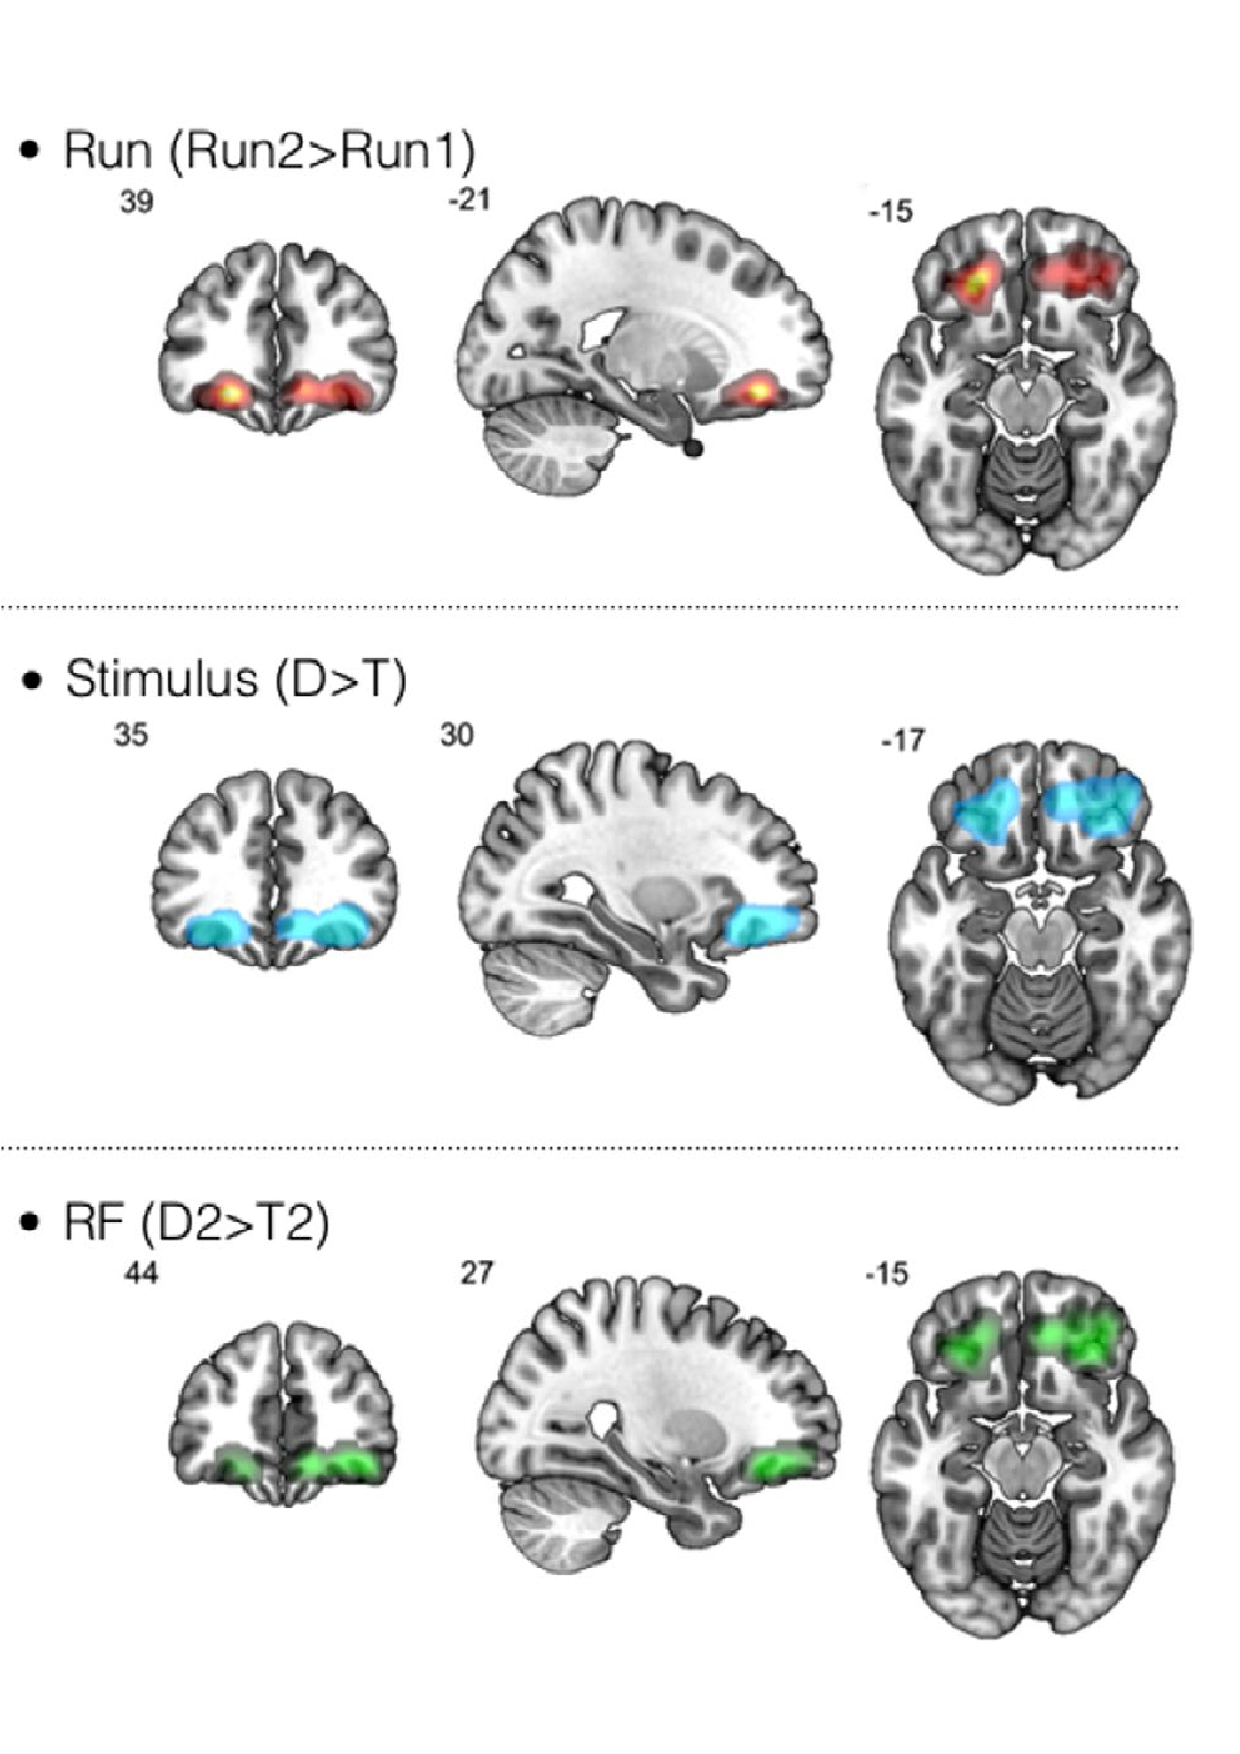
\includegraphics[width=0.7\linewidth]{images/Ch4/Figure5_voxelwise.pdf}
\caption{\textbf{Voxelwise contribution to each effect. } Brighter colours indicate a stronger contribution. D = Distractors; T = Target; D2 = Distractor stimuli during the second run; T2 = Target stimuli during the second run.} \label{fig:voxelwise}
\end{figure}




\subsection{Discussion}
With this study we assessed for the first time in a young population and using fMRI, the neural correlates of ORFi, a memory control mechanism crucial to maintain thoughts and behaviour in phase with reality.

Behaviourally, participants performed the test without difficulties, no differences in the accuracy were found, neither between the two types of stimuli (Distractors and Targets) nor between the two runs (1, 2). Moreover, the majority of participants performed well, making very few errors. This is similar to healthy adults, who had no difficulties to correctly perform the task even when runs were separated by only 1 minute \citep{Schnider1999, Wahlen2011}. Our results corroborate the idea that at this age ORFi is already an intuitive and efficacious cognitive process, corresponding to the storage capacity at that age \citep{Liverani2017}. 

Regarding reaction times, responses were slower in the second run of the task compared to the first run, reflecting the main challenge of the task, which is consistent with previous studies \citep{Bouzerda-Wahlen2015, Liverani2016, Liverani2017}. It appears that distinguishing between memories that are pertinent with the ongoing reality or not is more time consuming and takes more cognitive effort than simply recognising previously seen images. Our previous study assessing orbitofrontal reality filtering in children highlighted a significant difference between Distracters and Targets both for accuracy and reaction times \citep{Liverani2017}. In the current study participants were older, and they managed to distinguish almost perfectly between images seen in the current or in the previous run, performing at ceiling effect. Therefore, this could explain why no differences in accuracy and reaction time have been found between the two conditions. 

OFC activation was significantly stronger during the second run, which tests ORFi. Thus, our neuroimaging data in early adolescents were in line with lesion and imaging studies in adults, indicating that in this younger population, like in adults, the ORFi mechanism is needed to accomplish the second run of the task, and it is associated with specific OFC activation. Moreover, compared to Targets, OFC activation significantly increases in response to Distractors, stimuli that specifically require ORFi. Thus, using fMRI to explore ORFi for the first time, we confirmed previous findings showing that the ability to select information pertaining to the ongoing reality and to suppress irrelevant memory traces is associated with the activation of the OFC. 

Another added value of our study is that it extends these findings to a younger population: early adolescents aged between 10 and 13. Adolescence is a critical period in the development of the prefrontal cortex. There is a general consensus that the OFC – and the whole PFC – reaches complete maturity only at 20 years of age or more \citep{Diamond2002, Gogtay2004, Galvan2006}. Grey matter volume in the prefrontal cortex attains its maximal volume between 11 and 12 years old and then starts to decrease \citep{Giedd1999}, with a parallel improvement in cognitive functions such as source memory \citep{Sowell2001}. Given the late development of these prefrontal regions, one might speculate that the neural substrates of certain cognitive functions differ from early adolescence to adulthood. Nevertheless, our findings showing OFC activation while performing the reality filtering task in early adolescents of 10 to 13 years old indicate that this brain structure has matured enough to assume this function. 

The filtering of current irrelevant memories – that is, ORFi – bears conceptual resemblance with inhibitory control, defined as the ability to deliberately inhibit dominant, automatic or prepotent responses that are currently irrelevant \citep{Harnishfeger1995, StClair-Thompson2006}. According to \citeauthor{Schnider2018} (\citeyear{Schnider2018}), ORFi does not effectively  “inhibit” memories that are not pertinent with the ongoing reality, but it adapts their format, labelling and differentiating them as “fantasy” or “reality”. This process allows healthy individuals to then act differently and adequately according to fantasies or daydreams \citep{Nahum2009, Schnider2018}. Behavioural and neuroimaging data support this dissociation between ORFi and inhibitory control. Firstly, the ability to reject memories that are irrelevant to the present moment is already effective at the age of 7 \citep{Liverani2017} and does not correlate with behavioural inhibition measures, which is one of the last high-order functions to develop, continuing to consistently improve during adolescence \cite{Luna2010}. Secondly, the present study confirms that the neural basis of ORFi resides in the OFC already in 10-years old early adolescents. This finding corroborates the anatomical dissociation between the two mechanisms, since inhibition of unwanted memories has been associated with the activation of other prefrontal regions, such as dorsolateral prefrontal cortex, inferior frontal gyrus, and medio-temporal lobe \citep{Anderson2004, Luna2010}. 

In addition to being separate from inhibition processes, ORFi also needs to be differentiated from another memory monitoring ability, called source monitoring. Source monitoring is defined as the ability to accurately verify under which circumstances a memory has been acquired, and if it was self-generated or not \citep{Mitchell2009}. Previous studies demonstrated a behavioural and electrophysiological dissociation between the two mechanisms  \citep{Bouzerda-Wahlen2015}. Behaviourally, the retrieval of the source of a memory is a more demanding process compared to ORFi, as indicated by slower reaction times and higher error rates. Electrophysiologically, ORFi is characterised by a frontal positivity at 200-300 ms, while source monitoring is associated with a prolonged positivity from 400 ms on \citet{Bouzerda-Wahlen2015}. Unlike ORFi, the developmental trajectory of source monitoring is unclear: young children may be more prone than adult to confuse memories from different sources \citep{Lindsay1991}, but the debate is still open. Anatomically, different brain areas participate in source monitoring, including the precuneus \citep{Lundstrom2005}, the medial-temporal lobe \citep{Ross2008}, and the prefrontal cortex \citep{Mitchell2004, Mitchell2009} but not the OFC, specifically. Even if more whole-brain exploratory analyses would be needed, our results indicate a distinct activation pattern between ORFi and source monitoring. This corroborates the idea of the existence of two separate memory-monitoring mechanisms that dissociate at the behavioural, anatomical and electrophysiological level. 

Given the crucial importance of ORFi for the correct adaptation of behavioural demands in everyday life, it is of major interest to better investigate what is the impact of a deficit in this mechanism in other clinical populations characterised by lesions or atypical development in the OFC region. One promising field of research concerns schizophrenia, a psychiatric condition associated with loss of grey matter in this region. Indeed, recent studies showed that an abnormal ORFi activation can be an early biomarker of schizophrenia spectrum disorder \citep{Theze2019}. Another population characterised by specific alteration in the OFC region is preterm-born children \citep{Gimenez2006}. Up to now, no studies assessing the function of the OFC in the context of preterm birth have been done. Future research should address this point, using the paradigm assessing ORFi as a reliable task to explore OFC functions in premature children and adolescents. 

\subsection{Conclusion}

This research investigated for the first time using fMRI technique the neural correlates of orbitofrontal reality filtering in early adolescents. Results showed that, as in adults, the orbitofrontal cortex is involved in filtering memories and thoughts according to their relevance to the present in this young population. 







\subsection*{Acknowledgements}

This work was supported by the Swiss National Science Foundation (PI P.S. Hüppi, Number 324730\_163084) and the Fondation Campus Biotech Geneva (FCBG), a foundation of the Swiss Federal Institute of Technology Lausanne (EPFL), the University of Geneva (UniGe), and the Hôpitaux Universitaires de Genève (HUG). The authors thank Loan Mattera for her precious help in data acquisition and for her constructive suggestions.

\subsection*{Conflicts of interest}

We wish to confirm that there are no known conflicts of interest associated with this publication and there has been no significant financial support for this work that could have influenced its outcome. 

\subsection*{Data availability statement}

The data that support the findings of this study are available from the corresponding author upon reasonable request.



\newpage
\section{Journal Article: Altered orbitofrontal activation in preterm-born young adolescents during performance of a reality filtering task} \label{section:ch4_orfi_groups}

\begin{center}
 \textit{(Preprint or article to submit to Cerebral Cortex)}

Lorena G. A. Freitas\textsuperscript{1,2}, Maria Chiara Liverani\textsuperscript{1},  Vanessa Siffredi\textsuperscript{1,2}, Cristina Borradori Tolsa\textsuperscript{1}, Russia Ha-Vinh Leuchter\textsuperscript{1}, 
%Armin Schnider\textsuperscript{3},
Dimitri Van De Ville\textsuperscript{2}, Petra S. Hüppi\textsuperscript{1}



\end{center}

\textsuperscript{1} Department of Paediatrics, Gynecology and Obstetrics, Division of Development and Growth, Geneva University Hospitals, 6 rue Willy – Donzé, 1205 Geneva, Switzerland \\
\textsuperscript{2} Institute of Bioengineering, École Polytechnique Fédérale de Lausanne, Rue Cantonale, 1015 Lausanne, Switzerland  \\
%\textsuperscript{3} Department of Clinical Neurosciences, Division of Neurorehabilitation, Geneva University Hospitals, 26 Avenue de Beau-Séjour, 1211 Geneva, Switzerland  \\



\subsection*{Abstract}
Preterm birth --- that is, before 37 full weeks of gestational age --- is one of the predominant risk factors for neurodevelopmental problems, and has been associated with a wide range of impairments in cognitive functions spanning attention, working memory, executive functions, among others. Understanding the neurological underpinnings of these difficulties is crucial to identify potential interventions and establish critical periods to restore typical development. Indeed, neuroimaging studies have highlighted widespread alterations in regions such as the prefrontal cortex's structure and function in preterm individuals across lifetime. 

Reality filtering (RF) --- the ability to distinguish if a thought is relevant to present reality or not --- has been found to be mediated by the orbitofrontal cortex (OFC) in adults and typically developing early adolescents. Since this region is particularly vulnerable in individuals born prematurely, our aim was to investigate whether they rely on the OFC to complete an RF task. 

Here, we compare the neural correlates of Reality filtering in early adolescents born preterm with fullterm-born controls. Our findings indicate that the preterm group show lower activation of the OFC during performance of an RF task than controls, despite being able to successfully perform the task, with no significant increase in activation in other brain regions. This suggests that our preterm cohort have developed optimal mechanisms for reality filtering processing that do not require full activation of the OFC.

\textit{Keywords:} Preterm, Orbitofrontal Cortex, Reality Filtering; fMRI

\subsection{Introduction}



Preterm birth, defined as when delivery happens before 37 full weeks of gestational age (GA), affects an estimated 11.1\% of all live births every year \citep{Blencowe2013}.  
It has been associated with a wide range of impairments in cognitive functions and is one of the predominant risk factors for neurodevelopmental problems \citep{Twilhaar2018}, affecting attention \citep{Rommel2017}, working memory \citep{Allotey2018}, affective behaviour \citep{Hornman2016}, executive functions \citep{Costa2017, Burnett2018}, among others \citep{Moreira2014, Allotey2018}. Crucially, although some of these difficulties are often unveiled only when children reach school age, it has been shown that they may persist throughout life \citep{Anderson2014, Kajantie2019}. Therefore, understanding the neurological underpinnings of these difficulties is paramount to identify potential interventions and establish critical periods to restore typical development \citep{Wolke2019}.
    
One of the regions that deserve special attention in the context of the premature brain is the orbitofrontal cortex (OFC). It is crucial for a variety of complex and adaptive behaviors, such as affect recognition and emotional reappraisal \citep{Blair2000, Adolphs2001, Wager2008, Dixon2017}, assignment of value to a specific stimulus \citep{Montague2002}, prediction of specific outcomes \citep{Rudebeck2014}, reward processing \citep{Kahnt2018} and hedonic experiences \citep{KRINGELBACH2004}. Additionally, it is implicated in decision making \citep{Bechara2000,McClure2004}, social cognition and appropriate social behavior \citep{Rolls2004,Jonker2015} . As part of the prefrontal cortex, the OFC has a critical period of development in the last trimester of pregnancy \citep{Huttenlocher1997,Ruoss2001}. Consequently, OFC maturation is impacted by pretern birth, which usually takes place during this delicate period. The preterm brain can be characterized by brain volume reduction specifically in the OFC \citep{Thompson2007}. \citet{Gimenez2006} showed a reduction in the secondary sulci depth of the OFC, together with a reduced gray matter volume in the same region in very preterm children. \citet{Fischi-Gomez2015} found altered connectivity in the orbitofrontal and the medial network in extreme preterm children, and this weakness correlated with impaired social skills, simultaneous processing and hyperactivity. Cortical thickness in the frontal area, including OFC, has been correlated with internalizing and externalizing behavioral problems, common in premature children \citep{Zubiaurre-Elorza2012}. Finally, \citep{Ganella2015} found an altered distribution of the orbitofrontal sulcogyral folding pattern in adolescents born preterm, which correlated with deficits in executive functions. Taken together, all these data highlight the particular vulnerability of the OFC structure in the brain of individuals who were born prematurely.



While preterm birth has been shown by several neuroimaging studies to be linked to structural, functional and connectivity alterations in the prefrontal cortex \citep{Gimenez2006, Bjuland2013, Nosarti2014, Sripada2018}, to the best of our knowledge studies investigating OFC function are still missing in this context. The aim of our study was thus to fill this gap, using a task that specifically taps into this region while recording the functional activation of the brain in preterm-born young adolescents. 

In this study, we look into reality filtering (RF)  --- a memory-related mechanism that distinguishes if a thought is relevant to current reality or not. In adults \citep{Schnider2018} and in typically developing young adolescents aged 10-14 years old \citep{Liverani2020}, it is mediated by the OFC. Given this region's vulnerability in the preterm, we examined both whether this population is able to perform well in an RF task and, if this is the case, whether the OFC is also involved in this population, or a compensation mechanism has been put in place.  Finally, we compare the neural correlates of reality filtering (RF) in early adolescents born preterm with fullterm-born controls.

 
 \subsection{Methods}
 
\subsubsection{Participants} \label{subsection:PreVsCtrl_participants}
For this study, twenty-seven healthy term-born (TB) early adolescents from 10 to 14 years of age (12 females, mean age 12 $\pm$ 1.01 years) and thirty-seven age-matched preterm-born (PTB) individuals (20 females, mean age 12.1 $\pm$ 1.2 years) were recruited through advertisements. One TB participant was excluded due to strong signal distortions on fMRI images caused by the subject’s dental braces. One TB and two PTB participants were excluded due to high head-motion. Twenty-five TB and thirty-five PTB participants were finally included in the analysis.


Cognitive assessment at the time of the scan was performed in the same way as described in  \citet{Liverani2020}'s work (see Section \ref{subsection:OFC_participants}). Participants scored within the normal range of intellectual functioning (TB mean = 116.22 $\pm$ 11.33; PTB mean = 106.66 $\pm$ 11.98). Parents were asked to fill a questionnaire assessing the presence of serious physical illness or neurological problems. None of the participant had major disabilities, psychiatric or neurological diseases.

The Ethics Committee of the Canton of Geneva approved the study, which was carried out in accordance with the Declaration of Helsinki. Caregivers and participants provided informed written consent. All participants received a gift voucher of 100 Swiss francs for their participation in the study upon completion of the protocol. 


\subsubsection{fMRI Paradigm} 
All participants performed the reality filtering task described in section \ref{subsection:OFC_paradigm} and illustrated in Figure \ref{fig:taskDesign} \citep{Liverani2020}. In short, subjects performed two runs of an experiment in which a sequence of animal images were shown, and were asked to identify animals that had already been seen within the current run. Images shown for the first time within a run were called "Distractors (D)", while images seen for the second time within that same run were called "Target (T)". The set of images used in both runs were the same, meaning that the second run has the added difficulty of inhibiting the recognition of images seen in the previous run – the ability to perform the second run correctly is key for reality filtering. 

\subsubsection{Image acquisition} 
MRI data were recorded on a Siemens 3T Magnetom Prisma scanner at Campus Biotech, Geneva, Switzerland. Structural T1-weighted MP-RAGE (Magnetization Prepared Rapid Gradient Echo) sequences were acquired using the following parameters: voxel size = 0.9 x 0.9 x 0.9 mm; repetition time (TR)~=~2300 ms; echo time (TE) = 2.32 ms; inversion time (TI) = 900 ms; flip angle (FA)~=~8°; field of view (Fov) = 240 mm. Functional images were T2*-weighted with a multislice gradient-echo-planar imaging (EPI) sequence of 64 slices; voxel size = 2 x 2 x 2 mm; TR = 720 ms; TE = 33 ms; Fov = 208 mm. Finally, a fieldmap was acquired each time a participant entered the scanner, with TR = 627 ms; TE1 = 5.19 ms; TE2 = 7.65 ms; and FA = 60°.


\subsubsection{MRI data preprocessing} 
Our data were preprocessed using SPM12 (Wellcome Department of Imaging Neuroscience, UCL, UK) in MATLAB R2016a (The MathWorks, Inc., Natick, Massachusetts, United States) as in \citet{Liverani2020}. The fMRI images from each participant were spatially realigned and unwarped, respectively, to correct for motion artefacts and potential geometric distortions. The unwarping step brings two main advantages: it improves the co-registration between structural and functional images, and reduces the distortion variability across subjects during spatial normalization to a common space \citep{Hutton2002}. Functional images were then coregistered to structural images in subject space and smoothed with a Gaussian filter of full width at half maximum (FWHM) = 6 mm. To be able to perform a group level comparison, data were warped into MNI (Montreal Neurologic Institute) space via a study-specific DARTEL (Diffeomorphic Anatomical Registration using Exponentiated Lie algebra) template. Such normalisation methods have been shown to be robust to age differences in participants from the age of 7 \citep{ASHBURNER1998, Burgund2002}. In addition, including the DARTEL template as an intermediate step is among the top ranked currently available deformation algorithms \citep{Klein2009}.  


\subsubsection{Head motion} 
Head motion was assessed in terms of Framewise Displacement (FD; \citeauthor{Power2014a}, \citeyear{Power2014a}). One TB and two PTB subjects for whom more than 20\% of frames would be affected by motion (that is, frames with FD > 0.5 mm, one frame before, and two after those) were excluded. For the remaining subjects, total head motion was quite low in both groups: In the control group, for the first fMRI run the mean FD per frame was 0.159 mm with a standard deviation (SD) of $\pm$ 0.05 mm; for the second run the mean FD was 0.154 mm $\pm$ 0.05 mm; In the Preterm group, for the first fMRI run the mean FD per frame was 0.163 mm with a standard deviation (SD) of $\pm$ 0.05 mm; for the second run the mean FD was 0.165 mm $\pm$ 0.06 mm. The two groups did not significantly differ in mean FD neither for Run 1 (unpaired t-test, p = 0.74) nor for Run 2 (p = 0.54).

\subsubsection{fMRI analysis}
\textit{Whole brain analysis}: The fMRI data were analysed using SPM12 (Wellcome Department of Imaging Neuroscience, UCL, UK) in MATLAB R2016a (The MathWorks, Inc., Natick, Massachusetts, United States). For each subject, we built a first-level General Linear Model (GLM) including the condition (Distractor or Target images) regressors, as well as regressors of no interest that might affect the signal. Specifically, to account for effects potentially caused by head motion, we included in our model covariates-of-no-interest calculated in the following fashion: first, we computed the 24-parameter Volterra Expansion (VE) of the 6 motion parameters stored during the realignment step of the preprocessing pipeline. Secondly, we extracted the top 6 components (or those that explained 95\% of the variance in the VE) via singular value decomposition (SVD). Then, we included these components as nuisance regressors in the subject-level design matrix. This approach has been successfully used on our previous analyses of child data \citep{Adam-Darque2018, Liverani2020}. Finally, we employed the scan-nulling strategy \citep{Lemieux2007} to ignore information contained in fMRI images in which FD > 0.5mm, by adding extra regressors-of-no-interest for each of these time points. Finally, the results from this first-level analysis were included in a second-level factorial model including run and condition as factors. Statistical analysis was performed on a voxelwise basis searching for run, group, or interaction effects.



\textit{Region of interest (ROI) analysis}: Given the known involvement of the orbitofrontal cortex in the Reality filtering task studied here \citep{Schnider2018, Liverani2020}, we have delved deeper into the analysis of this area as a region of interest (ROI). To avoid confounding the results, the ROI we selected was based on a mask obtained from Neurosynth.org using a combination of 666 independent studies that included the OFC (for details of how the seed was created, see section \ref{section:OFC_ROIanal}). Group, run and condition effects were analysed using Student's t-tests. Interactions involving any combination of the three were analysed using a factorial analysis of variance (ANOVA).

\vspace{1cm}
\subsection{Results}

\subsubsection{Comparison of whole-brain activation during the two task runs}
In order to investigate general differences in activation between the two runs, we performed a second-level analysis where all the participants from both groups were pooled together. These results are depicted in Figure \ref{fig:RunActivation}. During performance of Run 2, three clusters were significantly more active than during Run 1. These are: right superior parietal lobule [MNI coordinates x = -54 y = -18 z = 49; p\textsubscript{FWE-corr} = 0.001], right amygdala [x = 21 y = -9 z = -18; p\textsubscript{FWE-corr} = 0.01], and left amygdala [x = -21 y = -9 z = -18; p\textsubscript{FWE-corr} = 0.02] – see Figure  \ref{fig:RunActivation}A. During performance of Run 1, the posterior parietal cortex was more activated [x = 0 y = -51 z = 20; p\textsubscript{unc} = 0.001]. This contrast can be seen in Figure \ref{fig:RunActivation}B.


\begin{figure}[h]
\centering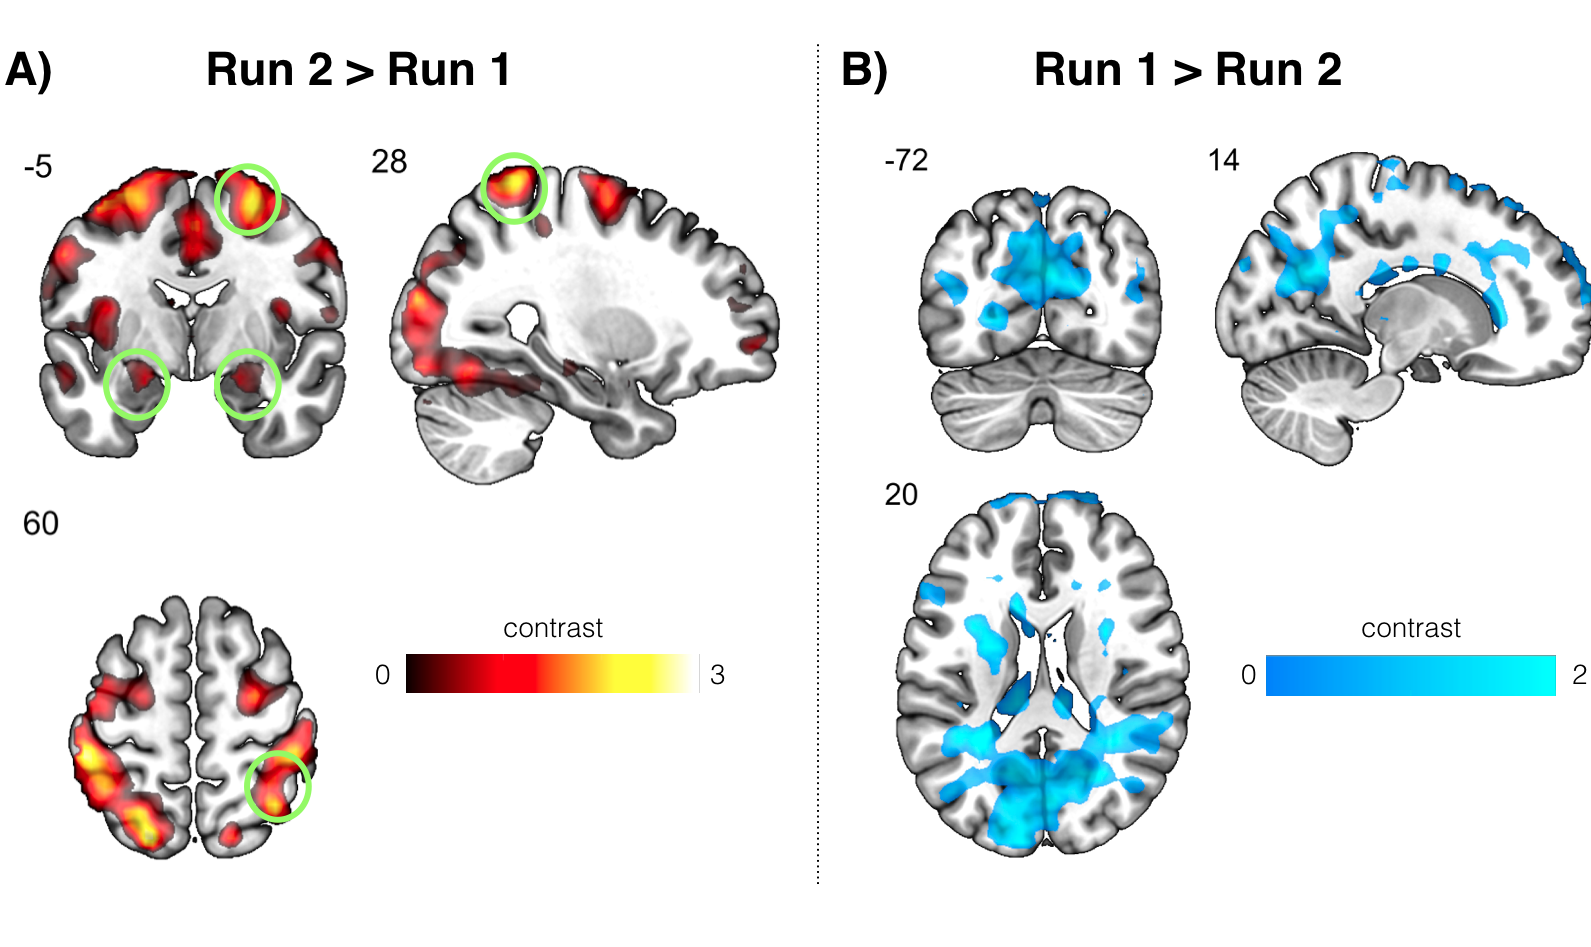
\includegraphics[width=1\linewidth]{images/Ch4/Ch4_CtrlVsPre_R1_R2.png}
\caption{\textbf{Comparison between the whole brain activation of the two runs.} The brain maps show regions that were most activated  (at $p < 0.001$), with subjects from both groups pooled together A)~During Run 2 (relevant for reality filtering), regions typically involved in external attention (\textit{e.g.}, superior parietal lobule) were more more activated than during Run 1. Green circles highlight regions that survived FWE correction at $\alpha$ = 0.05. \textit{Post hoc} analysis of activation during the two individual runs indicates that this difference is due to increased activation of these regions during Run 2, as opposed to decreased activity during Run 2.  B)~During Run 1, regions that typically form networks involved in  internally-oriented processes (\textit{e.g.}, default mode network) are more highly activated. \textit{Post hoc} analysis of activation during the two individual runs indicates that this difference is due to increased activation of these regions during Run 1. Note that no regions were significantly more active during Run 1 than during Run 2 after FWE correction.}  \label{fig:RunActivation}
\end{figure}

\subsubsection{Group comparison of whole-brain activation during the two task runs}

We next sought to identify whether there was a group difference in activation during performance of the task runs. These results are illustrated in Figure  \ref{fig:GroupActivation}. Term-born controls had higher activation of the medial temporal gyrus (MNI coordinates x = -39 y = -39 z = 9; $p = 0.001$, \textit{unc}) and the right orbitofrontal cortex (x = 21 y = 42 z = -9; $p_{\text{FWE-corr}} = 0.02$). \textit{Post hoc} analysis of activation during the two individual runs indicates that this difference is due to increased activation of these regions in the Term-born group, as opposed to decreased activity in the preterm group (not shown). Preterm participants showed higher activation in visual attention areas (x = 40 y = -74 z = 20; $p_{\text{FWE-corr}} = 0.04$) and motor areas related to finger movement (x = -42 y = -39  z = 66; $p_{\text{FWE-corr}} = 0.04$) as compared to controls. \textit{Post hoc} analysis of activation during the two individual runs indicates that this difference is due to increased activation of motor regions in the Preterm group, and decreased activation in attention areas in the Term-Born group.


\begin{figure}[h]
\vspace{3mm}
\centering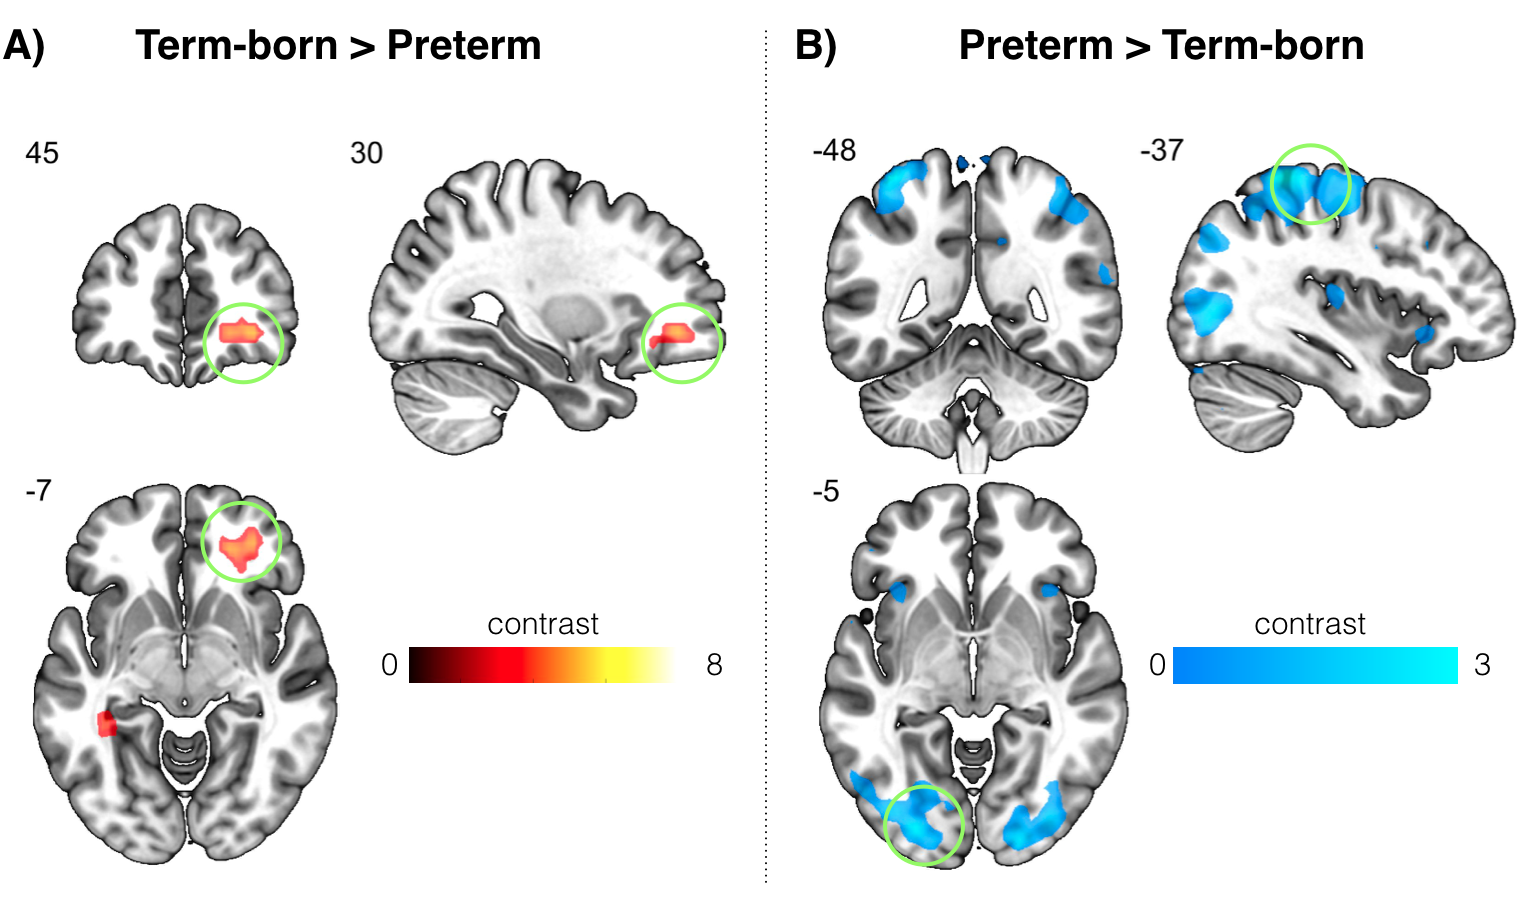
\includegraphics[width=1\linewidth]{images/Ch4/Ch4_CtrlVsPre_ctrl_pre.png}
\caption{\textbf{Group differences in activation across the two runs.} The brain maps show regions that were most activated at height threshold $p = 0.001$, with maps from both runs pooled together. Green circles highlight regions that survived FWE correction at $\alpha$ = 0.05. A)~Term-born controls had higher activation of the medial temporal gyrus (MNI coordinates x = -39 y = -39 z = 9; $p = 0.001$, \textit{unc}) and the right orbitofrontal cortex (x = 21 y = 42 z = -9; $p_{\text{FWE-corr}} = 0.02$). B)~Preterm participants showed higher activation in visual attention areas (x = 40 y = -74 z = 20; $p_{\text{FWE-corr}} = 0.04$) and motor areas related to finger movement (x = -42 y = -39  z = 66; $p_{\text{FWE-corr}} = 0.04$).} \label{fig:GroupActivation}
\end{figure} 

\vspace{0.5cm}
\subsubsection{Interactions between group and run effects}

A group versus run interaction contrast identified several clusters as depicted in Figure \ref{fig:Interaction}. They include the orbitofrontal cortex (x = 15 y = 39  z = -6; $p = 0.001$), nodes of the frontoparietal network such as dorsolateral prefrontal cortex and posterior parietal cortex (x = -24 y = 30  z = 48; $p = 0.001$), insula (x = -43 y = -3  z = -15; $p = 0.001$) and visual attention areas (x = -27 y = -63  z = 21; $p = 0.001$). A \textit{post hoc} comparison between the two runs in the two groups separately revealed that these differences are mainly due to increased activation of these regions during the second run in the control group (Figure \ref{fig:Interaction}, right).

\begin{figure}[h]
\vspace{3mm}
\centering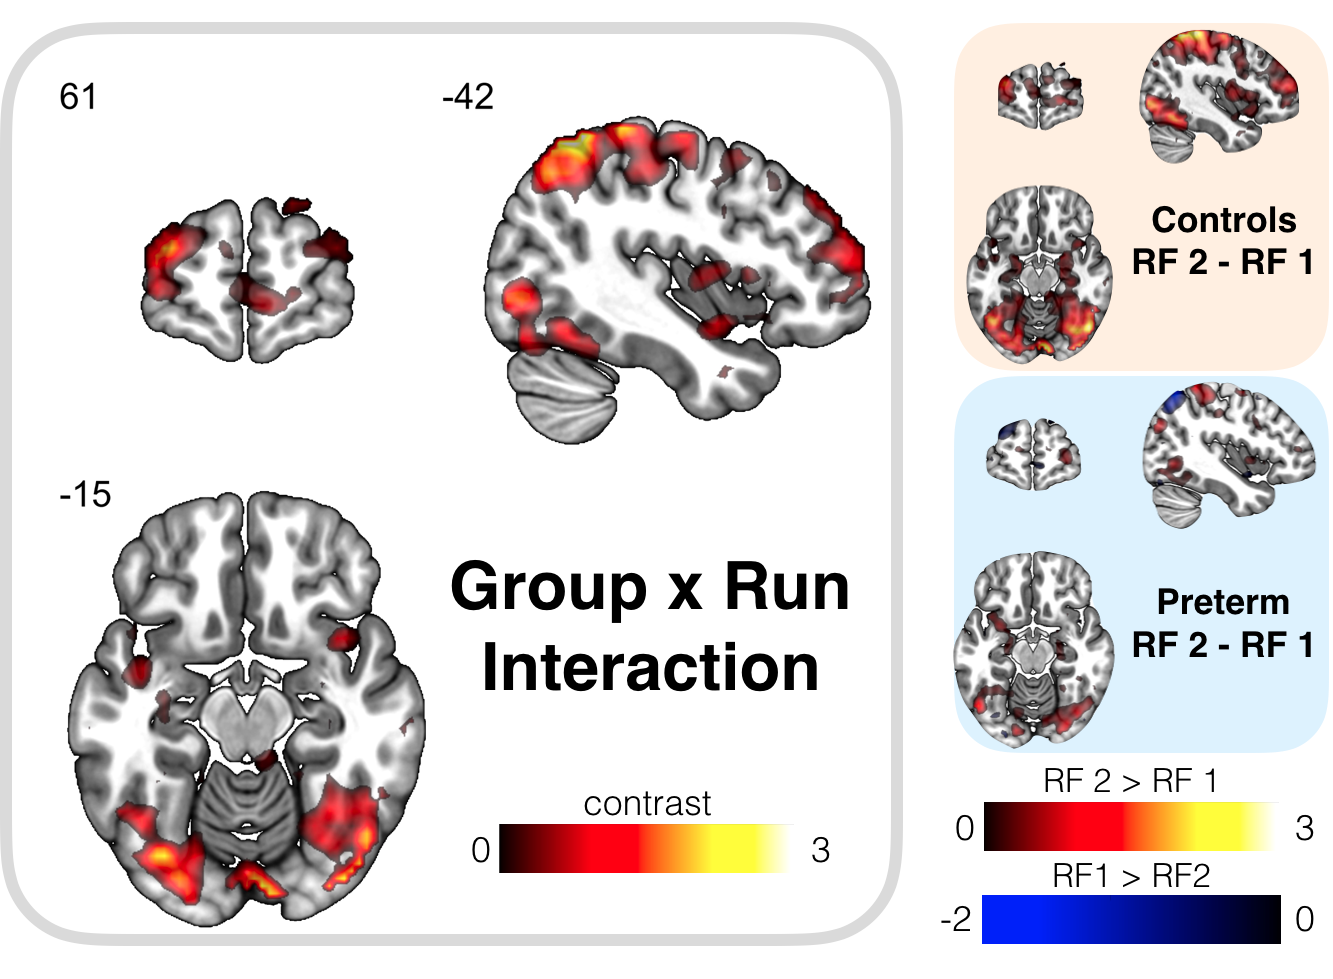
\includegraphics[width=1\linewidth]{images/Ch4/Ch4_CtrlVsPre_interaction.png}
\caption{\textbf{Group versus Run interaction effects.} (Left) The brain maps show regions whose activation showed an interaction of Group and Run effects at height threshold $p = 0.001$. (Right, orange inset) Contrast between the two runs in the Control group. Red areas indicate higher activation during Run 2 (RF 2), while blue regions indicate higher activation during Run 1 (RF 1). (Right, blue inset) Contrast between the two runs in the preterm group. Red areas indicate higher activation during Run 2, while blue regions indicate higher activation during Run 1.}
 \label{fig:Interaction}
\end{figure}


\vspace{1cm}
\subsubsection{Orbitofrontal cortex as an ROI}
An ROI analysis focused on the orbitofrontal cortex (OFC) revealed a Run effect (t = 2.47, $p = 0.007$), where the activation during Run 2 was higher than during Run 1 and a tendency for a Group effect (t~=~1.4, $p = 0.05$). Finally, OFC activation during presentation of Distractor images in the reality filtering run (RF2) was higher in controls than in preterm-born individuals (t~= ~2.38, $p = 0.01$ ). The ANOVA analysis revealed the interactions shown in Figure \ref{fig:ch4_ROI_Interactions}. OFC activation was higher in both groups during performance of the second run (RF 2), and higher in the fullterm-born (Control) group than in the preterm-born group during both runs, but the difference in activation between the two runs was larger in the Control group, as indicated by the steeper slope of the yellow line in the Run vs. Group interaction plot from Figure \ref{fig:ch4_ROI_Interactions}. Blood oxygenation level dependent (BOLD) signal was stronger during the presentation of both types of stimuli (Distractor, D; and Target, T) during the second run, and the difference in activation between runs was larger for stimuli of the Target type, as shown by the red dotted line in the Stimulus vs. Run interaction plot from Figure \ref{fig:ch4_ROI_Interactions}. Finally, the control group has a much steeper increase in activation during presentation of Distractor stimuli from moments when Target stimuli where presented, as compared to their preterm peers (orange dotted line in the Group vs. Stimulus interaction plot from Figure \ref{fig:ch4_ROI_Interactions}). The difference in activation between groups was higher for Distractor images than for Target images (green full line in the Stimulus vs. Group plot from Figure \ref{fig:ch4_ROI_Interactions}). None of the interactions were statistically significant, but the trends identified here are discussed in the next session.


\begin{figure}[h]
%\vspace{3mm}
\centering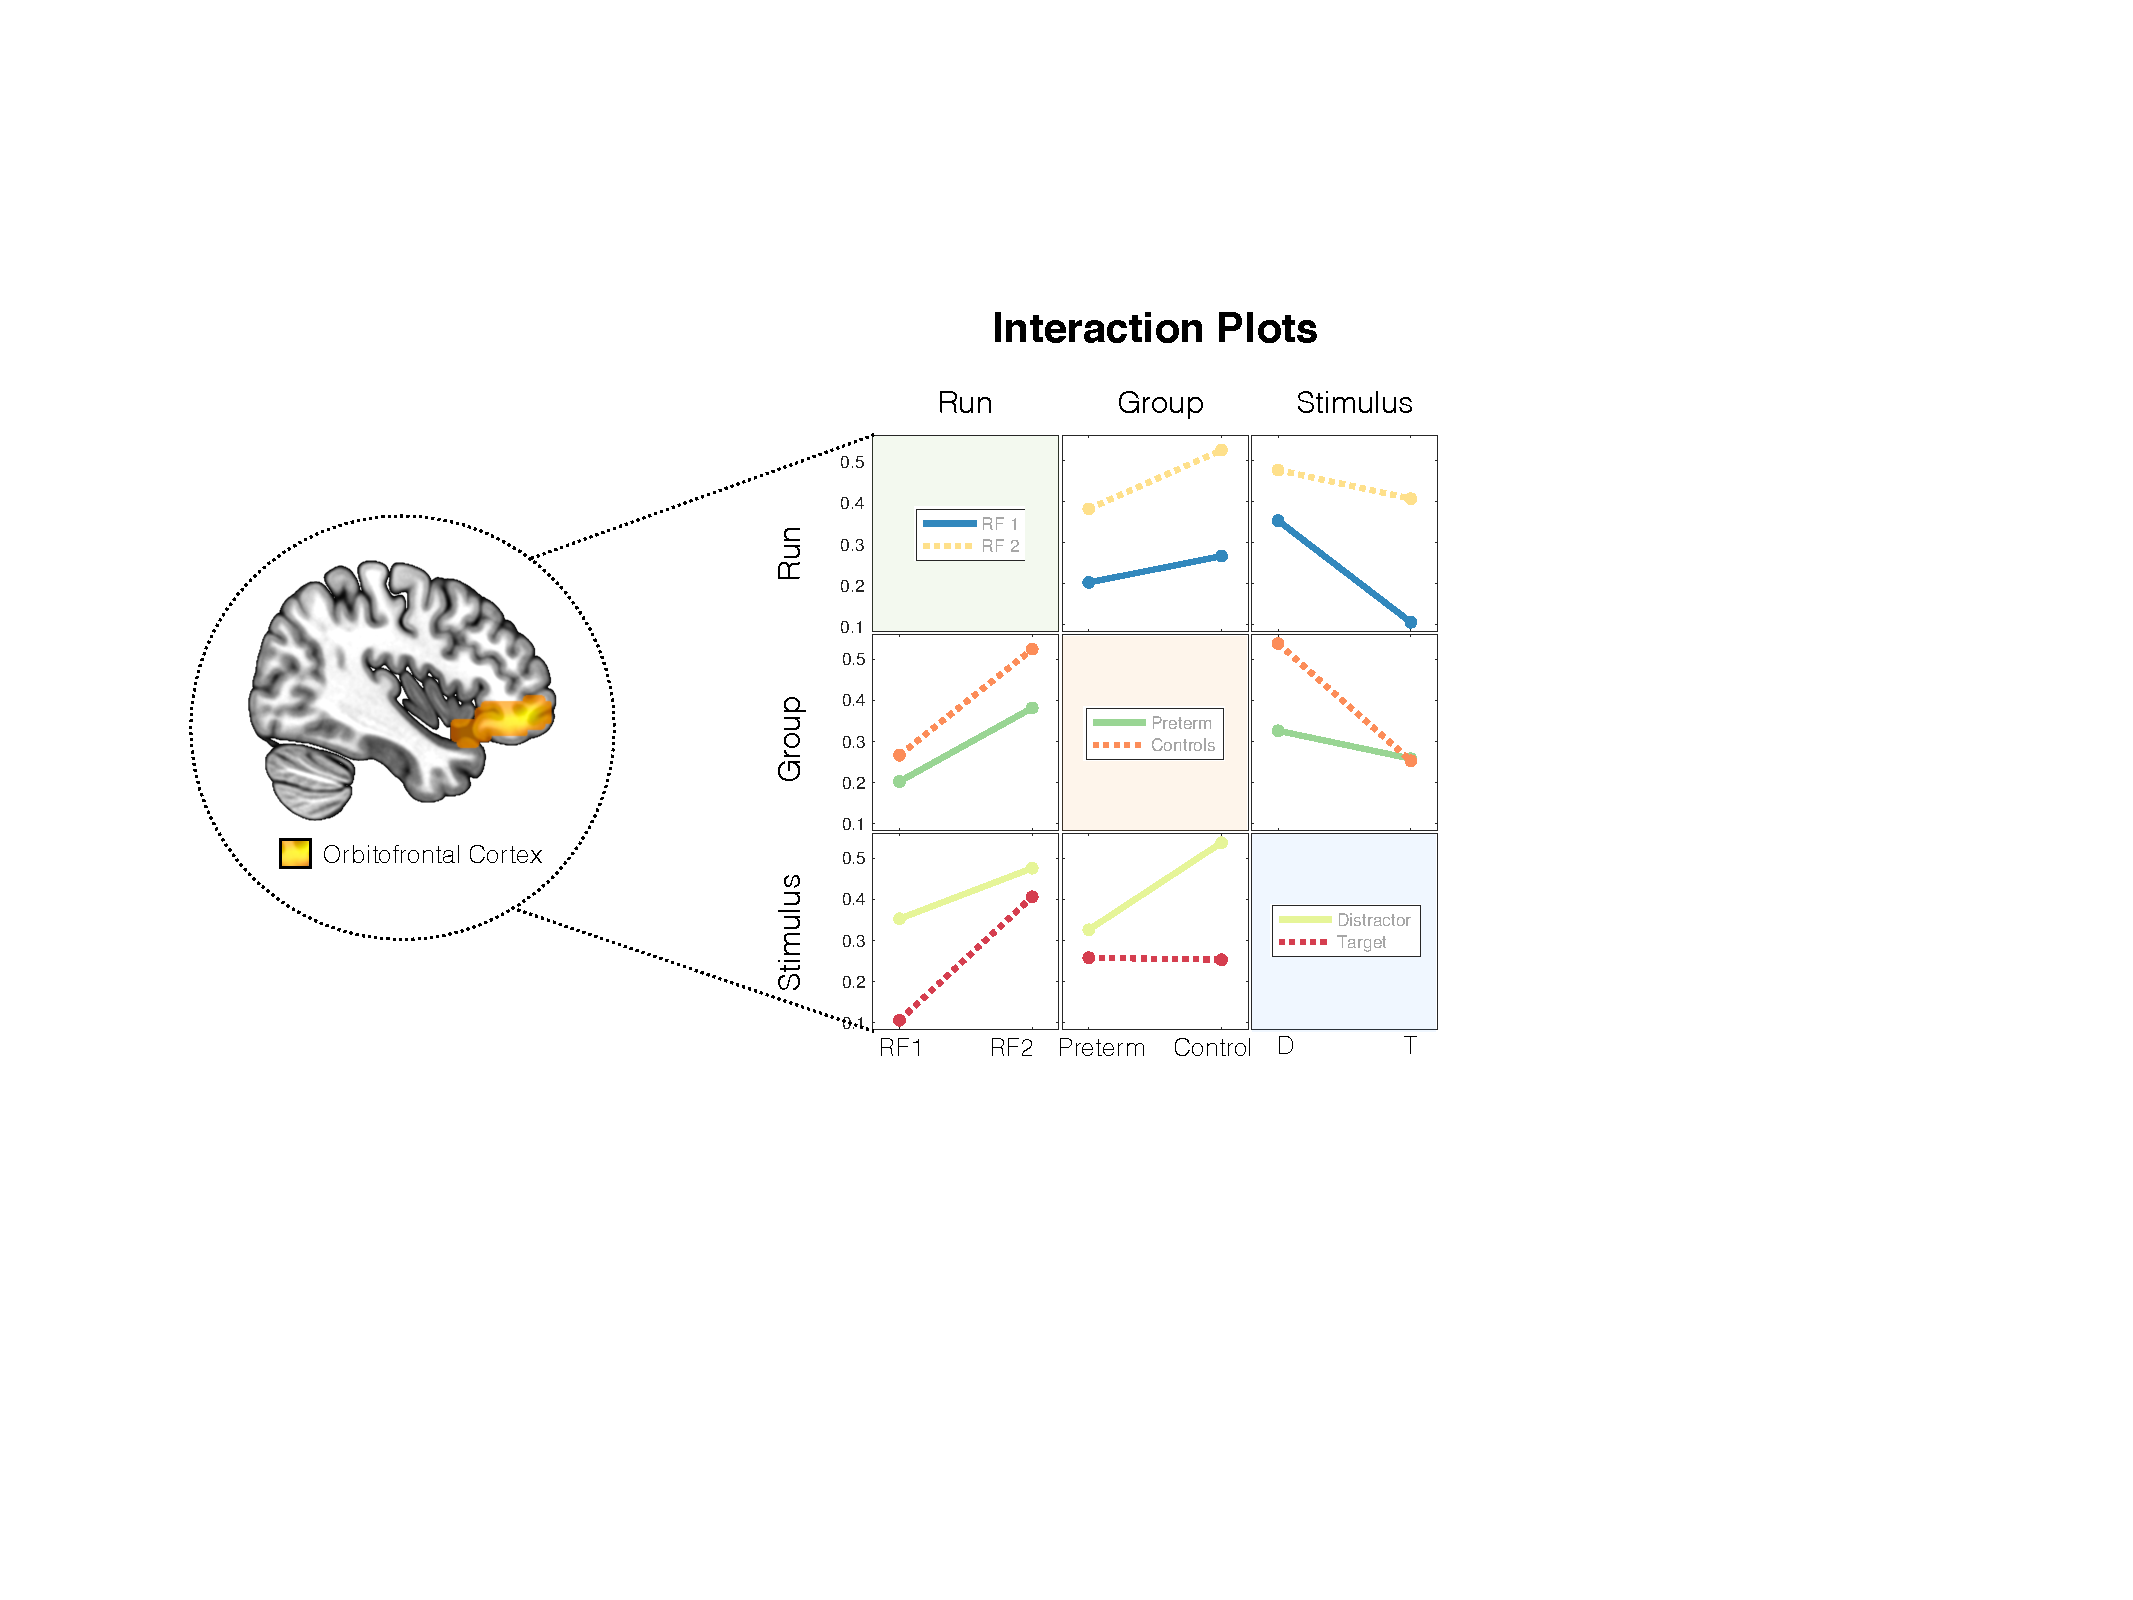
\includegraphics[width=1\linewidth]{images/Ch4/Ch4_ROI_Interactions.pdf}
\caption{\textbf{Group, Run and Stimulus interaction effects in activation of the orbitofrontal cortex as a region of interest.} (Left) The orbitofrontal cortex (sagittal plane with MNI coordinate x = 40). (Right)~Interaction plots involving runs, groups and stimulus types. The y-axis of all plots represent the average BOLD signal for the corresponding factor (\textit{e.g.}, run, group or stimulus). } \label{fig:ch4_ROI_Interactions}
\end{figure} 







\subsection{Discussion}

\subsubsection{Comparison of whole-brain activation during the two task runs}

 During performance of the first run of the experiment, the activation of regions typically involved in internally-oriented attention (\textit{i.e.}, nodes of the default mode network such as the posterior parietal cortex) tended to be higher in comparison to during the second run of the experiment. Given that the same set of images is used for both runs, Run 2 (RF 2) is significantly harder than Run 1. This is because, in Run 2, subjects must not only recognise images that were already seen during the current run, but also suppress memories from the previous one. The fact that the activation of these areas is higher during the first run is thus in line with previous studies which found that default mode network activation is inversely proportional to task demand \citep{Ceko2015}. This finding may be interpreted as a greater occurrence of moments of introspection or mind-wandering during Run 1 given the ease of the task, which is reflected in the ceiling effect found in the participants' responses.

Run 2, in turn, requires more effort since participants must not only recognise  images that have already been seen during the current run, but also filter the memory of those images that have only been already seen during the first run. It is thus not surprising that brain regions related to attentional control and information manipulation during working memory-related tasks \citep{Koenigs2009, Wu2016} are more highly activated during this run. 

Finally, the areas more highly activated during either of the runs are not specific to the task we are studying: in fact, they have been widely found to be part of well-known networks which are involved in other cognitive tasks and / or present during the resting state \citep{VandenHeuvel2010a}. This is not surprising given that we pooled participants from both groups together for this part of the analysis ––– if they evoke different brain regions to perform the task, these results could be expected to be averaged out when all subjects are grouped together. Our results so far may thus suggest that either participants from the two groups use different underlying mechanisms to perform the reality filtering task, or at least that the level of activation in these two groups differs, decreasing the power to find these task-specific regions.

\subsubsection{Group comparison of whole-brain activation during the two task runs}
We found significant differences in activation during the performance of the reality filtering task when comparing the two groups. We identified increased activation of the orbitofrontal cortex in Term-Born young adolescents as compared to their Preterm-Born peers. By itself, this result could have been achieved under three scenarios: 1) high activation of the OFC in the control group during task performance; 2) de-activation of the OFC in the preterm group; 3) or a combination of the two.  The \textit{post hoc} analysis of the individual groups indicated that the first hypothesis is true: this difference is due to high activation of the OFC in the Term-Born participants. The high activation of OFC in the control group is inline with previous work that identify the OFC as a mediator of Reality Filtering in healthy populations \citep{Schnider2000, Treyer2003,Bouzerda-Wahlen2015, Schnider2018, Theze2019}, including our own previous work on healthy young adolescents \citep{Liverani2020}. Failure to process reality filtering functions has been a consistent marker of reality confusion in clinical patients with damage in the OFC or in structures directly connected to it \citep{Schnider1999, Nahum2012}. The fact that the preterm individuals did not activate the OFC as highly may be linked to previous findings of delayed development of frontal areas in this population \citep{Nosarti2014, Sripada2018}. However, that they are still able to perform the task despite lower activation in the OFC can mean one of two things: either they have developed a more efficient way of performing the same task that requires less use of this region, or the lack of development of this area has been compensated by other processes. This is further discussed in the next subsection.

Preterm young adolescents had significantly higher activation in motor areas related to finger movement than their Term-Born counterparts. This difference was due to an increase in activation in these areas in the preterm, rather than de-activation in the control group. While this may seem unexpected, given that all participants performed both runs of the task by clicking mouse buttons with the right hand fingers, it is in line with previous research \citep{Heep2009, Arichi2010, Allievi2016}. \citet{Heep2009} and  \citet{Arichi2010} found in separate studies that unilateral motor stimulation led to bilateral activation of the sensorimotor cortex in preterm infants. In our results, regions related to visual attention were also more active in the Preterm than in the control group. This was surprising, since nodes of the attention network have been consistently found to be less active in the preterm population \citep{Olsen2018}. Our inspection of the contrast values for individual groups revealed that this was due to decreased activation of attention-related ares in the control group. This is probably due to the fact that the task was too easy, which is in line with the ceiling effect we observed in the participants' answers.

\subsubsection{Interactions between whole-brain group and run effects}
Although the two runs of our experiment have the same instruction (\textit{i.e.}, to identify images that were repeated during the current run), it is during the second run that reality filtering processing is required. This is because during Run 2, while recognising images as already seen, participants must also decide whether those have been already seen during the current run or only the previous one. Thus, investigating interactions between group and run effects was important for us to further understand what aspects of reality filtering were really different between groups. Although the results from this analysis did not survive multiple comparison correction, they point towards a few interesting trends. For instance, the dorsolateral prefrontal cortex and posterior parietal cortices were more highly activated in the control group during Run 2. These regions are key nodes of the frontoparietal network, which is crucial for the ability to coordinate behaviour in a flexible, accurate and timely manner \cite{Marek2018}. This may justify fullterm-born children's ability to respond more quickly to the task (Liverani et al., 2020b, in preparation) \add{Did I make this up? I seem to remember this was the case but can't be sure}. In addition, the control group showed higher increase in orbitofrontal cortex activation during the second run than the preterm-born individuals. This in itself is not surprising, given that preterm birth is known to be linked to altered development of frontal structure, function and connectivity \citep{Sripada2018}. Interestingly, however, young adolescents born preterm were able to perform the task successfully with a low rate of errors. This may be due to different hypotheses. Firstly, there may be a compensatory mechanism involving other parts of the brain that allow the preterm group to perform the task through different routes. However, no brain areas were significantly more active in this population than in the control group during the second run. An alternative possibility is that the preterm group does indeed rely on the orbitofrontal cortex to perform the task and that, given the alterations in frontal cortices, have developed a more efficient way to perform the task that optimises OFC activation. Finally, since there was a ceiling effect in the accuracy of the responses from both groups, this could be due to the task having been too easy for this age. Our results indicate the second or third options as potential explanations. However, as discussed in Section \ref{sub:limitations} (Challenges and Limitations), further studies involving a more difficult version of the task would help clarify this issue. 

\subsubsection{Group, Run and Stimulus interaction effects on OFC activation}
Given the known role of the OFC in mediating reality filtering processing, we performed additional analyses using this area as a region of interest. Although the results were not statistically significant (and we discuss the possible reasons in Section  \ref{sub:limitations}), the trends we found were extremely interesting, and we chose to report them to serve as a base for future studies. For instance, while the fact that OFC activation was higher in both groups during performance of Run 2, and higher in the fullterm-born (Control) group than in the preterm-born group during both runs agrees with our whole-brain results, this analysis illustrates that the difference in activation between the two runs was larger in the Control group. 

BOLD signal in the OFC was stronger in general during the second run independently of the type of stimulus, and the increase in activation was higher for stimuli of the Distractor type rather than of the Target type. This is in line with previous research indicating that the role of the OFC in reality filtering relates to suppressing memories that are not currently relevant (thus while processing images of the Distractor type during Run 2) \citep{Schnider2018}.  Further, the control group shows a larger increase in activation during presentation of Distractor stimuli from moments when Target stimuli where presented, as compared to their preterm peers. Since the young adolescents that were born preterm were able to perform the task with high accuracy, this suggests that this group have found an optimal way to process this function that does not require activation of the OFC to the same levels as typically developing children.


\subsubsection{Challenges and Limitations} \label{sub:limitations}
 As described before, a ceiling effect in the participants from both groups' responses, such that nearly no mistakes were ever made, preventing us from being able to investigate potential correlations between brain activation and accuracy levels. This effect may have been due to the fact that we used the same task that had been described as used for children from 7 years of age. It is thus possible that we have missed higher activation of regions involved in the processing of this task. Future studies involving young adolescents should thus increase the difficulty of the task by methods such as increasing the number of trials, shortening the time for individual trials, and / or adding different types of distractor elements (\textit{e.g.}, images never repeated during Run 1 that reappear during Run 2, and images that appear for the first time in Run 2). Although there is room for improvement, this study sheds important light into differences between reality filtering processing in individuals born preterm or at term and presents avenues for future research.
%The fact that both runs of the experiment use the same set of images means that Reality Filtering-specific results may be confounded by brain activations caused by performing the exercise a second time. We believe this is not a significant problem since, at the time the second run starts, all images have been seen for the exact number of times, and the goal during this run is different from the first one. Nonetheless, future studies should include a set of images that are never repeated during the first run, but only repeated during the second run. 

\subsection{Conclusion}
In this study, we investigated the neurological underpinnings of a reality filtering task performance in young adolescents born prematurely as compared to their term-born peers. We identified differences in activation in the two groups while performing the two steps of the task and framed them within previous knowledge on preterm birth and reality filtering processing. Our results corroborate the idea that compensatory mechanisms are in place to make up for preterm birth-related difficulties, allowing individuals to perform functional tasks. Such results may be used as biomarkers for future studies on potential interventions to help this population. 



\subsection*{Acknowledgements}
This work was supported by the Swiss National Science Foundation, grant no. 324730-163084 to PSH. The authors thank Loan Mattera, Roberto Martuzzi and Greta Mikneviciute for their help in data acquisition. 

\subsection*{Conflict of Interest Statement}
The authors declare that the research was conducted in the absence of any commercial or financial relationships that could be construed as a potential conflict of interest.




\begin{comment}
In this chapter we will see some examples of mathematics.

Here's an example how to cite.~\cite{atc13}

\lipsum[1]

\section{Very important formulas}
\lipsum[2]

\begin{equation}\label{eqn:rate_eqns}
\frac{\textrm{d}}{\textrm{d}t}\left[
\begin{array}{l}
P_{\textit{0}} \\
P_{\textit{1}} \\
P_{\textit{T}}
\end{array}
\right] =
\left[
\begin{array}{l}
\frac{P_{\textit{1}}}{\tau_{\textit{10}}} + \frac{P_{\textit{T}}}{\tau_{\textit{T}}} - \frac{P_{\textit{0}}}{\tau_{\textit{ex}}} \\
- \frac{P_{\textit{1}}}{\tau_{\textit{10}}} - \frac{P_{\textit{1}}}{\tau_{isc}} + \frac{P_{\textit{0}}}{\tau_{\textit{ex}}} \\
\frac{P_{\textit{1}}}{\tau_{isc}} -  \frac{P_{\textit{T}}}{\tau_{\textit{T}}}
\end{array}
\right]
\end{equation}

\lipsum[3]


\begin{equation}\label{eqn:avgfluorescence}
\bar{I_{f}}(\vec{r})
	= \gamma(\vec{r}) \left(1 - \frac{\tau_{\textit{T}} P_{\textit{T}}^{{eq}}\left(1-\exp \left(-\frac{(T_p - t_p)}{\tau_{\textit{T}}}\right)\right)}{1-\exp\left(-\frac{(T_p - t_p)}{\tau_{\textit{T}}} + k_{\textit{2}} t_p\right)} \times \frac{\left(\exp\left(k_{\textit{2}} t_p\right)-1\right)}{t_p} \right)
\end{equation}

\lipsum[3]
\end{comment}